\documentclass{tufte-book}

\usepackage{tikz}
\usetikzlibrary{arrows, positioning}
\usepackage{mathrsfs}
\usepackage{pgffor}
\usepackage{enumitem}
\usepackage{graphics}
\usepackage{algorithm2e}
\usepackage{hyperref}
\hypersetup{
  colorlinks=true,
  linkcolor=red,
  citecolor=green,
  filecolor=magenta,
  urlcolor=cyan
}

\usepackage{color}
\definecolor{mybackground}{RGB}{204, 232, 207}
\pagecolor{mybackground}

\usepackage{amsmath, amssymb, amsthm}
\newtheorem{THM}{Theorem}[section]
\newtheorem{DEF}{Definition}[section]
\newtheorem{LEM}{Lemma}[section]
\newtheorem{PROP}{Proposition}[section]
\newtheorem{CORO}{Corollary}[section]
\newtheorem{FACT}{Fact}[section]
\newtheorem{CLAIM}{Claim}[section]
\newtheorem{OBSER}{Observation}[section]
\newtheorem{remark}{Remark}[section]
\newcommand\numberthis{\addtocounter{equation}{1}\tag{\theequation}}
% left foot mark for math symbol
\usepackage{leftidx}

\usepackage{tcolorbox}
\newtcolorbox{thmbox}[3][]
{
  colframe = #2!25,
  colback  = #2!10,
  coltitle = #2!20!black,  
  title    = {#3},
  #1,
}
\newenvironment{theorem}[1][]{
  \begin{thmbox}{blue}{
      \begin{THM}
        #1
      \end{THM}
  }
  \it
}{
  \end{thmbox}
}
\newenvironment{define}[1][]{
  \begin{thmbox}{green}{
      \begin{DEF}
        #1
      \end{DEF}
  }
}{
  \end{thmbox}
}
\newenvironment{lemma}[1][]{
  \begin{thmbox}{black}{
      \begin{LEM}
        #1
      \end{LEM}
  }
  \it
}{
  \end{thmbox}
}

\newenvironment{proposition}[1][]{
  \begin{thmbox}{orange}{
      \begin{PROP}
        #1
      \end{PROP}
  }
}{
  \end{thmbox}
}
\newenvironment{corollary}[1][]{
  \begin{thmbox}{black}{
      \begin{CORO}
        #1
      \end{CORO}
  }
}{
  \end{thmbox}
}
\newenvironment{fact}[1][]{
  \begin{thmbox}{orange}{
      \begin{FACT}
        #1
      \end{FACT}
  }
}{
  \end{thmbox}
}

\newenvironment{claim}[1][]{
  \begin{thmbox}{black}{
      \begin{CLAIM}
        #1
      \end{CLAIM}
  }
}{
  \end{thmbox}
}

\newenvironment{observation}[1][]{
  \begin{thmbox}{blue}{
      \begin{OBSER}
        #1
      \end{OBSER}
  }
}{
  \end{thmbox}
}

% mark the words in tikz
\newcommand{\MK}[3][]{
  \tikz [remember picture, baseline, #1]
  \node (#2) [anchor = base, minimum size = 0mm, inner sep = 0mm] {#3};
}

% mark the words in tikz in math mode
\newcommand{\MKM}[3][]{
  \tikz [remember picture, baseline, #1]
  \node (#2) [anchor = base, minimum size = 0mm, inner sep = 0mm] {$#3$};
}

% mark the words in tikz (with a counter)
\newcount\markcnt
\markcnt=0
\newcommand{\MKN}[2][]{
  \advance\markcnt by 1
  \tikz [remember picture, baseline, #1]
  \node (\the\markcnt) [anchor = base, minimum size = 0mm, inner sep = 0mm] {#2};
}
% mark the words in tikz (with a counter) in math mode
\newcommand{\MKNM}[2][]{
  \advance\markcnt by 1
  \tikz [remember picture, baseline, #1]
  \node (\the\markcnt) [anchor = base, minimum size = 0mm, inner sep = 0mm] {$#2$};
}

\usepackage{makeidx}
\makeindex

\title{\Huge Notes for Jerrum Book}
\author{Xiaoyu Chen}

% add depth for table of contents
\addtocontents{toc}{\protect\setcounter{tocdepth}{2}}

% set counter for sections and theorems environment
\setcounter{secnumdepth}{2}

\begin{document}
\maketitle
\tableofcontents
\clearpage

\chapter{Topics Related to Markov Chain}
\clearpage

% time reversible markov chain
\section{Coupling From the Past}
\paragraph{}
Coupling from the past (CFTP) is a method with which we could perform a perfect sampling according to some distribution.
I can not find any convincing proof of this result, so I decide to prove it myself.

First, lets view Markov Chain in a new but nature way.
Suppose we have a Markov Chain $\mathcal{M}$ defined on some state set $S = \{s_1, s_2, \cdots, s_n\}$.
Note that when we execute $\mathcal{M}$, then in each turn, this chain will fix some parameters according to some distribution and move from some states to other states.
So, if we fix this random parameters, then $\mathcal{M}$ becomes a determined process, and we could view it as a function $f: S\to S$. For convenience, lets denote the determined process from time $i$ to time $i+1$ by $f_i$.
The pseudocode of CFTP is shown below.
\begin{algorithm}
  Coupling From The Past () \Begin{
    $T \gets 1$ \\
    \Repeat{$f$ becomes a constant function}{
      $f \gets f_{-T} \circ f_{-(T-1)} \circ \cdots \circ f_{-1}$ \\
      $T \gets T + 1$
    }
    \Return{$f(s_1)$}
  }
\end{algorithm}
\marginnote[-3cm]{The $\circ$ here means compose operator where $f \circ g  (x) = g(f(x))$, i.e. give $f$'s output as $g$'s input.}
\marginnote[-1.8cm]{Here, $f_{-i}$ is fixed (by random) at the first time we encountered it, and will be \textbf{reused} later.}

The idea of this sampler is quite simple.
Suppose we have a Markov Chain $\mathcal{M}$ which starts at $-\infty$ and stops at $0$, then its pretty sure that it will have the distribution $\pi$ at time $0$ (no matter which state it starts from).
Then, if we randomly determine some last finite steps of the chain (say $T$ steps), we may have the chance to recover the sample of this MC by this steps.

And, its quite easy to see that when the last $T$ steps forms a constant function we could easily recover the sample from this MC. So we have the following theorem:
\begin{theorem}
  If we have a Markov Chain $\mathcal{M}$ such that
  \[\lim_{t\to\infty} \Pr [f_0 \circ f_1 \circ \cdots \circ f_t \mbox{ is a constant function}] = 1\]
  where $f_0, f_1, \cdots, f_t$ are fixed randomly according to the transition matrix $P$ of $\mathcal{M}$,
  then the CFTP of $\mathcal{M}$ halt in finite time with probability $1$ and returns a sample according to $\pi$.
\end{theorem}
\begin{proof}
  Note that, if our algorithm could \textbf{cover} all the cases of the last finite steps of the Markov Chain, and could \textbf{recover} the sample from all these cases, then its easy to see, this algorithm should be right.

  So, here, its quite nature to ask, what means all the cases?
  Here, a case is a suffix of the chain from $-\infty$ to $0$.
  Note that, CFTP randomly choose a $f_{-t}$ at time $-t$, so if we omit the stop condition, its should cover all the cases.
  Suppose the CFTP stops at some time $T$, which means its forms a constant function $f$ and no matter how we extend this suffix, this constant will not change, so we could pack all the suffix that end with this suffix into this suffix, since they have the same sample (while do not change the distribution of sample).
  Hence, CFTP forms a cover of all the cases.

  Since $\lim_{t\to\infty}\Pr[f_0\circ f_1\circ \cdots\circ f_t] = 1$, the Markov Chain will be a constant function with probability 1 after infinite steps. Which notes us that CFTP should halt in finite time with probability $1$.
  
  Finally, since CFTP simulates a Markov Chain which have been executed for infinite steps, so the distribution of the sample should be exactly $\pi$.
\end{proof}

\subsection{Two confusing bad variations of CFTP}
\paragraph{Coupling to the future}
Its nature for us to ask, ``why not just coupling to the future?'', since this two samplers look nearly the same.
\begin{algorithm}
  Copuling To The Future () \Begin{
    $T\gets 1$ \\
    \Repeat{$f$ becomes a constant function}{
      $f \gets f_0\circ f_1\circ \cdots \circ f_T$ \\
      $T\gets T+1$
    }
    \Return{$f(s_1)$}
  }
\end{algorithm}

The problem here is that is sampler does not cover all the cases.
First, if we omit the stop condition, then it is easy to see that this sampler covers all the cases. Similarly, this sampler want to pack some of the cases so that we could stop in finite steps. Note that, if $f$ becomes a constant function in time $T$, then $f'$ will also be a constant function in time $T+1$ and so on. But $f$ and $f'$ has different constant, so we could not pack them together (we should not use the sample of $f$ to represent the sample of $f'$).
So, there is a bias in the result distribution.

Here is a quite simple example to explain this:
Suppose we have a Markov chain with state space $[2] = \{1, 2\}$ and transition matrix
\[P = \left[
    \begin{array}{cc}
      0.5 & 0.5 \\
      1   & 0
    \end{array}
  \right]\]
Obviously, $\pi = (\pi_1, \pi_2) = (\frac{2}{3}, \frac{1}{3})$.
In this example, the \emph{coupling to the future} sampler always returns $1$ as its result.

\begin{center}
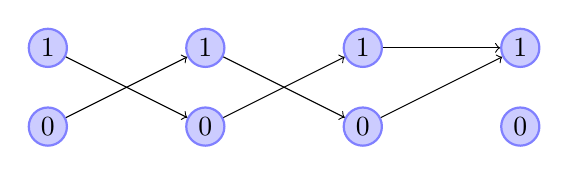
\begin{tikzpicture}
  [state/.style={circle, draw=blue!50, fill=blue!20, thick, inner sep=2pt}]
  \foreach \x in {0, 2, 4, 6}{
    \node (n1\x) at (\x, 1) [state] {1};
    \node (n0\x) at (\x, 0) [state] {0};
  }
  \draw [->] (n10) to (n02);
  \draw [->] (n00) to (n12);
  \draw [->] (n12) to (n04);
  \draw [->] (n02) to (n14);
  \draw [->] (n14) to (n16);
  \draw [->] (n04) to (n16);
\end{tikzpicture}
\end{center}

\paragraph{Coupling From The Past with no Memory}
It is quite nature to implement the CFTP sampler without \textbf{reuse}, but unfortunately, this variation of CFTP is wrong.
This sampler covers all the cases, but it does not follow the right distribution.
The probobility of this sampler returns sample $s$ equals:
\begin{align*}
&\sum_{T=1}^\infty \Pr[\mbox{$f$ has constant $s$ $|$ $\substack{\mbox{$f$ is a constant function in $T$}\\ \mbox{$\land$ $f$ is not a constant function in $\{1, \cdots, T-1\}$}}$}] \\
                  &= \sum_{T=1}^\infty \Pr[\mbox{$f$ has constant $s$ $|$ sampler halts in $T$ steps}] \Pr[\mbox{sampler halts in $T$ steps}] \\
  &= \sum_{T=1}^\infty \frac{\Pr[\mbox{constant function in $T$ steps with constant $s$}]}{\Pr[\mbox{function in $T$ steps}]} \prod_{t=1}^{T-1}\frac{\Pr[\mbox{$t$ steps not constant function}]}{\Pr[\mbox{function in $t$ steps}]} \\
\end{align*}
Actually, its hard to find any relationship between this distribution and the correct distribution.
When $s = 1$, then using the example above, we have
\begin{align*}
  \Pr[s = 1] &\geq \textcolor{red}{\Pr[\mbox{1 step}]}\textcolor{blue}{\Pr[\mbox{$f$ has constant $1$} | \mbox{1 step}]} + \textcolor{cyan}{\Pr[\mbox{2 steps}]}\textcolor{blue!50}{\Pr[\mbox{$f$ has constant $1$} | \mbox{2 steps}]} \\
             &= \textcolor{red}{\frac{1}{2}}\cdot \textcolor{blue}{1} + \textcolor{cyan}{\frac{1}{2}\cdot\frac{3}{4}}\cdot\textcolor{blue!50}{\frac{2}{3}} \\
  &= \frac{3}{4} > \frac{2}{3}
\end{align*}
So, its easy to see that this sampler does not catch the right distribution.

\begin{center}
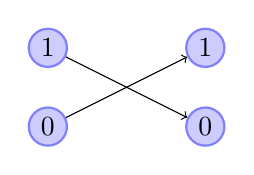
\begin{tikzpicture}
  [state/.style={circle, draw=blue!50, fill=blue!20, thick, inner sep=2pt}]
  \foreach \x in {0, 2}{
    \node (n1\x) at (\x, 1) [state] {1};
    \node (n0\x) at (\x, 0) [state] {0};
  }
  \draw [->] (n10) to (n02);
  \draw [->] (n00) to (n12);
\end{tikzpicture} \hspace{0.5cm}
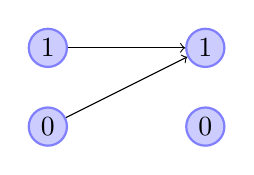
\begin{tikzpicture}
  [state/.style={circle, draw=blue!50, fill=blue!20, thick, inner sep=2pt}]
  \foreach \x in {0, 2}{
    \node (n1\x) at (\x, 1) [state] {1};
    \node (n0\x) at (\x, 0) [state] {0};
  }
  \draw [->] (n10) to (n12);
  \draw [->] (n00) to (n12);
\end{tikzpicture}
\end{center}

\begin{center}
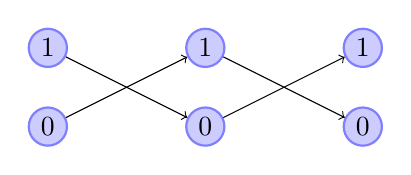
\begin{tikzpicture}
  [state/.style={circle, draw=blue!50, fill=blue!20, thick, inner sep=2pt}]
  \foreach \x in {0, 2, 4}{
    \node (n1\x) at (\x, 1) [state] {1};
    \node (n0\x) at (\x, 0) [state] {0};
  }
  \draw [->] (n10) to (n02);
  \draw [->] (n00) to (n12);
  \draw [->] (n12) to (n04);
  \draw [->] (n02) to (n14);
\end{tikzpicture} \hspace{0.5cm}
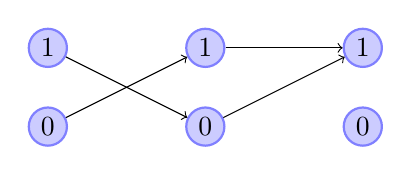
\begin{tikzpicture}
  [state/.style={circle, draw=blue!50, fill=blue!20, thick, inner sep=2pt}]
  \foreach \x in {0, 2, 4}{
    \node (n1\x) at (\x, 1) [state] {1};
    \node (n0\x) at (\x, 0) [state] {0};
  }
  \draw [->] (n10) to (n02);
  \draw [->] (n00) to (n12);
  \draw [->] (n12) to (n14);
  \draw [->] (n02) to (n14);
\end{tikzpicture} \vspace{0.5cm} \\
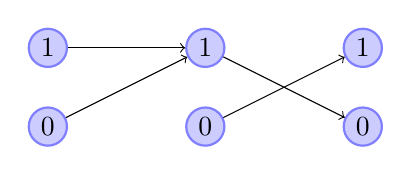
\begin{tikzpicture}
  [state/.style={circle, draw=blue!50, fill=blue!20, thick, inner sep=2pt}]
  \foreach \x in {0, 2, 4}{
    \node (n1\x) at (\x, 1) [state] {1};
    \node (n0\x) at (\x, 0) [state] {0};
  }
  \draw [->] (n10) to (n12);
  \draw [->] (n00) to (n12);
  \draw [->] (n12) to (n04);
  \draw [->] (n02) to (n14);
\end{tikzpicture} \hspace{0.5cm}
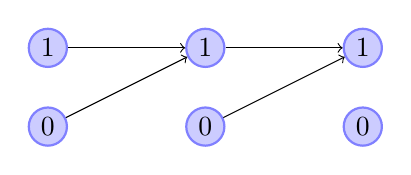
\begin{tikzpicture}
  [state/.style={circle, draw=blue!50, fill=blue!20, thick, inner sep=2pt}]
  \foreach \x in {0, 2, 4}{
    \node (n1\x) at (\x, 1) [state] {1};
    \node (n0\x) at (\x, 0) [state] {0};
  }
  \draw [->] (n10) to (n12);
  \draw [->] (n00) to (n12);
  \draw [->] (n12) to (n14);
  \draw [->] (n02) to (n14);
\end{tikzpicture} 
\end{center}
%%% Local Variables:
%%% mode: latex
%%% TeX-master: "../../notebook"
%%% End:


% how to use markov chain to simulate a specific distribution
\section{Coupling From the Past}
\paragraph{}
Coupling from the past (CFTP) is a method with which we could perform a perfect sampling according to some distribution.
I can not find any convincing proof of this result, so I decide to prove it myself.

First, lets view Markov Chain in a new but nature way.
Suppose we have a Markov Chain $\mathcal{M}$ defined on some state set $S = \{s_1, s_2, \cdots, s_n\}$.
Note that when we execute $\mathcal{M}$, then in each turn, this chain will fix some parameters according to some distribution and move from some states to other states.
So, if we fix this random parameters, then $\mathcal{M}$ becomes a determined process, and we could view it as a function $f: S\to S$. For convenience, lets denote the determined process from time $i$ to time $i+1$ by $f_i$.
The pseudocode of CFTP is shown below.
\begin{algorithm}
  Coupling From The Past () \Begin{
    $T \gets 1$ \\
    \Repeat{$f$ becomes a constant function}{
      $f \gets f_{-T} \circ f_{-(T-1)} \circ \cdots \circ f_{-1}$ \\
      $T \gets T + 1$
    }
    \Return{$f(s_1)$}
  }
\end{algorithm}
\marginnote[-3cm]{The $\circ$ here means compose operator where $f \circ g  (x) = g(f(x))$, i.e. give $f$'s output as $g$'s input.}
\marginnote[-1.8cm]{Here, $f_{-i}$ is fixed (by random) at the first time we encountered it, and will be \textbf{reused} later.}

The idea of this sampler is quite simple.
Suppose we have a Markov Chain $\mathcal{M}$ which starts at $-\infty$ and stops at $0$, then its pretty sure that it will have the distribution $\pi$ at time $0$ (no matter which state it starts from).
Then, if we randomly determine some last finite steps of the chain (say $T$ steps), we may have the chance to recover the sample of this MC by this steps.

And, its quite easy to see that when the last $T$ steps forms a constant function we could easily recover the sample from this MC. So we have the following theorem:
\begin{theorem}
  If we have a Markov Chain $\mathcal{M}$ such that
  \[\lim_{t\to\infty} \Pr [f_0 \circ f_1 \circ \cdots \circ f_t \mbox{ is a constant function}] = 1\]
  where $f_0, f_1, \cdots, f_t$ are fixed randomly according to the transition matrix $P$ of $\mathcal{M}$,
  then the CFTP of $\mathcal{M}$ halt in finite time with probability $1$ and returns a sample according to $\pi$.
\end{theorem}
\begin{proof}
  Note that, if our algorithm could \textbf{cover} all the cases of the last finite steps of the Markov Chain, and could \textbf{recover} the sample from all these cases, then its easy to see, this algorithm should be right.

  So, here, its quite nature to ask, what means all the cases?
  Here, a case is a suffix of the chain from $-\infty$ to $0$.
  Note that, CFTP randomly choose a $f_{-t}$ at time $-t$, so if we omit the stop condition, its should cover all the cases.
  Suppose the CFTP stops at some time $T$, which means its forms a constant function $f$ and no matter how we extend this suffix, this constant will not change, so we could pack all the suffix that end with this suffix into this suffix, since they have the same sample (while do not change the distribution of sample).
  Hence, CFTP forms a cover of all the cases.

  Since $\lim_{t\to\infty}\Pr[f_0\circ f_1\circ \cdots\circ f_t] = 1$, the Markov Chain will be a constant function with probability 1 after infinite steps. Which notes us that CFTP should halt in finite time with probability $1$.
  
  Finally, since CFTP simulates a Markov Chain which have been executed for infinite steps, so the distribution of the sample should be exactly $\pi$.
\end{proof}

\subsection{Two confusing bad variations of CFTP}
\paragraph{Coupling to the future}
Its nature for us to ask, ``why not just coupling to the future?'', since this two samplers look nearly the same.
\begin{algorithm}
  Copuling To The Future () \Begin{
    $T\gets 1$ \\
    \Repeat{$f$ becomes a constant function}{
      $f \gets f_0\circ f_1\circ \cdots \circ f_T$ \\
      $T\gets T+1$
    }
    \Return{$f(s_1)$}
  }
\end{algorithm}

The problem here is that is sampler does not cover all the cases.
First, if we omit the stop condition, then it is easy to see that this sampler covers all the cases. Similarly, this sampler want to pack some of the cases so that we could stop in finite steps. Note that, if $f$ becomes a constant function in time $T$, then $f'$ will also be a constant function in time $T+1$ and so on. But $f$ and $f'$ has different constant, so we could not pack them together (we should not use the sample of $f$ to represent the sample of $f'$).
So, there is a bias in the result distribution.

Here is a quite simple example to explain this:
Suppose we have a Markov chain with state space $[2] = \{1, 2\}$ and transition matrix
\[P = \left[
    \begin{array}{cc}
      0.5 & 0.5 \\
      1   & 0
    \end{array}
  \right]\]
Obviously, $\pi = (\pi_1, \pi_2) = (\frac{2}{3}, \frac{1}{3})$.
In this example, the \emph{coupling to the future} sampler always returns $1$ as its result.

\begin{center}
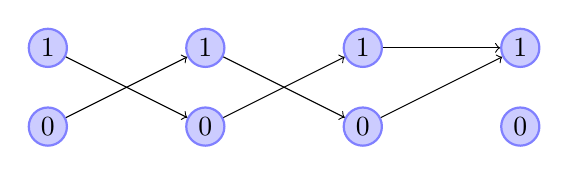
\begin{tikzpicture}
  [state/.style={circle, draw=blue!50, fill=blue!20, thick, inner sep=2pt}]
  \foreach \x in {0, 2, 4, 6}{
    \node (n1\x) at (\x, 1) [state] {1};
    \node (n0\x) at (\x, 0) [state] {0};
  }
  \draw [->] (n10) to (n02);
  \draw [->] (n00) to (n12);
  \draw [->] (n12) to (n04);
  \draw [->] (n02) to (n14);
  \draw [->] (n14) to (n16);
  \draw [->] (n04) to (n16);
\end{tikzpicture}
\end{center}

\paragraph{Coupling From The Past with no Memory}
It is quite nature to implement the CFTP sampler without \textbf{reuse}, but unfortunately, this variation of CFTP is wrong.
This sampler covers all the cases, but it does not follow the right distribution.
The probobility of this sampler returns sample $s$ equals:
\begin{align*}
&\sum_{T=1}^\infty \Pr[\mbox{$f$ has constant $s$ $|$ $\substack{\mbox{$f$ is a constant function in $T$}\\ \mbox{$\land$ $f$ is not a constant function in $\{1, \cdots, T-1\}$}}$}] \\
                  &= \sum_{T=1}^\infty \Pr[\mbox{$f$ has constant $s$ $|$ sampler halts in $T$ steps}] \Pr[\mbox{sampler halts in $T$ steps}] \\
  &= \sum_{T=1}^\infty \frac{\Pr[\mbox{constant function in $T$ steps with constant $s$}]}{\Pr[\mbox{function in $T$ steps}]} \prod_{t=1}^{T-1}\frac{\Pr[\mbox{$t$ steps not constant function}]}{\Pr[\mbox{function in $t$ steps}]} \\
\end{align*}
Actually, its hard to find any relationship between this distribution and the correct distribution.
When $s = 1$, then using the example above, we have
\begin{align*}
  \Pr[s = 1] &\geq \textcolor{red}{\Pr[\mbox{1 step}]}\textcolor{blue}{\Pr[\mbox{$f$ has constant $1$} | \mbox{1 step}]} + \textcolor{cyan}{\Pr[\mbox{2 steps}]}\textcolor{blue!50}{\Pr[\mbox{$f$ has constant $1$} | \mbox{2 steps}]} \\
             &= \textcolor{red}{\frac{1}{2}}\cdot \textcolor{blue}{1} + \textcolor{cyan}{\frac{1}{2}\cdot\frac{3}{4}}\cdot\textcolor{blue!50}{\frac{2}{3}} \\
  &= \frac{3}{4} > \frac{2}{3}
\end{align*}
So, its easy to see that this sampler does not catch the right distribution.

\begin{center}
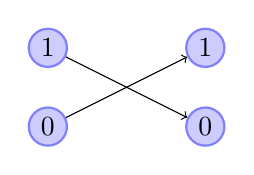
\begin{tikzpicture}
  [state/.style={circle, draw=blue!50, fill=blue!20, thick, inner sep=2pt}]
  \foreach \x in {0, 2}{
    \node (n1\x) at (\x, 1) [state] {1};
    \node (n0\x) at (\x, 0) [state] {0};
  }
  \draw [->] (n10) to (n02);
  \draw [->] (n00) to (n12);
\end{tikzpicture} \hspace{0.5cm}
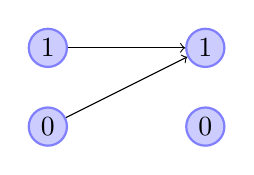
\begin{tikzpicture}
  [state/.style={circle, draw=blue!50, fill=blue!20, thick, inner sep=2pt}]
  \foreach \x in {0, 2}{
    \node (n1\x) at (\x, 1) [state] {1};
    \node (n0\x) at (\x, 0) [state] {0};
  }
  \draw [->] (n10) to (n12);
  \draw [->] (n00) to (n12);
\end{tikzpicture}
\end{center}

\begin{center}
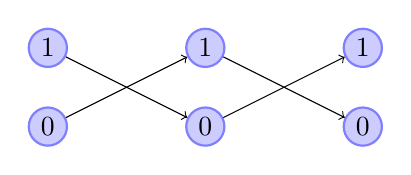
\begin{tikzpicture}
  [state/.style={circle, draw=blue!50, fill=blue!20, thick, inner sep=2pt}]
  \foreach \x in {0, 2, 4}{
    \node (n1\x) at (\x, 1) [state] {1};
    \node (n0\x) at (\x, 0) [state] {0};
  }
  \draw [->] (n10) to (n02);
  \draw [->] (n00) to (n12);
  \draw [->] (n12) to (n04);
  \draw [->] (n02) to (n14);
\end{tikzpicture} \hspace{0.5cm}
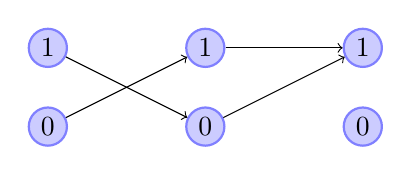
\begin{tikzpicture}
  [state/.style={circle, draw=blue!50, fill=blue!20, thick, inner sep=2pt}]
  \foreach \x in {0, 2, 4}{
    \node (n1\x) at (\x, 1) [state] {1};
    \node (n0\x) at (\x, 0) [state] {0};
  }
  \draw [->] (n10) to (n02);
  \draw [->] (n00) to (n12);
  \draw [->] (n12) to (n14);
  \draw [->] (n02) to (n14);
\end{tikzpicture} \vspace{0.5cm} \\
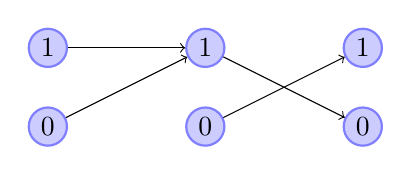
\begin{tikzpicture}
  [state/.style={circle, draw=blue!50, fill=blue!20, thick, inner sep=2pt}]
  \foreach \x in {0, 2, 4}{
    \node (n1\x) at (\x, 1) [state] {1};
    \node (n0\x) at (\x, 0) [state] {0};
  }
  \draw [->] (n10) to (n12);
  \draw [->] (n00) to (n12);
  \draw [->] (n12) to (n04);
  \draw [->] (n02) to (n14);
\end{tikzpicture} \hspace{0.5cm}
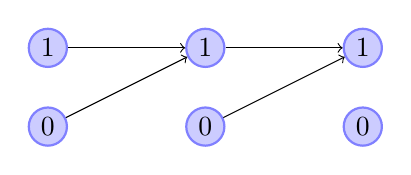
\begin{tikzpicture}
  [state/.style={circle, draw=blue!50, fill=blue!20, thick, inner sep=2pt}]
  \foreach \x in {0, 2, 4}{
    \node (n1\x) at (\x, 1) [state] {1};
    \node (n0\x) at (\x, 0) [state] {0};
  }
  \draw [->] (n10) to (n12);
  \draw [->] (n00) to (n12);
  \draw [->] (n12) to (n14);
  \draw [->] (n02) to (n14);
\end{tikzpicture} 
\end{center}
%%% Local Variables:
%%% mode: latex
%%% TeX-master: "../../notebook"
%%% End:


% some useful tricks for using trnasition matrix
\section{Coupling From the Past}
\paragraph{}
Coupling from the past (CFTP) is a method with which we could perform a perfect sampling according to some distribution.
I can not find any convincing proof of this result, so I decide to prove it myself.

First, lets view Markov Chain in a new but nature way.
Suppose we have a Markov Chain $\mathcal{M}$ defined on some state set $S = \{s_1, s_2, \cdots, s_n\}$.
Note that when we execute $\mathcal{M}$, then in each turn, this chain will fix some parameters according to some distribution and move from some states to other states.
So, if we fix this random parameters, then $\mathcal{M}$ becomes a determined process, and we could view it as a function $f: S\to S$. For convenience, lets denote the determined process from time $i$ to time $i+1$ by $f_i$.
The pseudocode of CFTP is shown below.
\begin{algorithm}
  Coupling From The Past () \Begin{
    $T \gets 1$ \\
    \Repeat{$f$ becomes a constant function}{
      $f \gets f_{-T} \circ f_{-(T-1)} \circ \cdots \circ f_{-1}$ \\
      $T \gets T + 1$
    }
    \Return{$f(s_1)$}
  }
\end{algorithm}
\marginnote[-3cm]{The $\circ$ here means compose operator where $f \circ g  (x) = g(f(x))$, i.e. give $f$'s output as $g$'s input.}
\marginnote[-1.8cm]{Here, $f_{-i}$ is fixed (by random) at the first time we encountered it, and will be \textbf{reused} later.}

The idea of this sampler is quite simple.
Suppose we have a Markov Chain $\mathcal{M}$ which starts at $-\infty$ and stops at $0$, then its pretty sure that it will have the distribution $\pi$ at time $0$ (no matter which state it starts from).
Then, if we randomly determine some last finite steps of the chain (say $T$ steps), we may have the chance to recover the sample of this MC by this steps.

And, its quite easy to see that when the last $T$ steps forms a constant function we could easily recover the sample from this MC. So we have the following theorem:
\begin{theorem}
  If we have a Markov Chain $\mathcal{M}$ such that
  \[\lim_{t\to\infty} \Pr [f_0 \circ f_1 \circ \cdots \circ f_t \mbox{ is a constant function}] = 1\]
  where $f_0, f_1, \cdots, f_t$ are fixed randomly according to the transition matrix $P$ of $\mathcal{M}$,
  then the CFTP of $\mathcal{M}$ halt in finite time with probability $1$ and returns a sample according to $\pi$.
\end{theorem}
\begin{proof}
  Note that, if our algorithm could \textbf{cover} all the cases of the last finite steps of the Markov Chain, and could \textbf{recover} the sample from all these cases, then its easy to see, this algorithm should be right.

  So, here, its quite nature to ask, what means all the cases?
  Here, a case is a suffix of the chain from $-\infty$ to $0$.
  Note that, CFTP randomly choose a $f_{-t}$ at time $-t$, so if we omit the stop condition, its should cover all the cases.
  Suppose the CFTP stops at some time $T$, which means its forms a constant function $f$ and no matter how we extend this suffix, this constant will not change, so we could pack all the suffix that end with this suffix into this suffix, since they have the same sample (while do not change the distribution of sample).
  Hence, CFTP forms a cover of all the cases.

  Since $\lim_{t\to\infty}\Pr[f_0\circ f_1\circ \cdots\circ f_t] = 1$, the Markov Chain will be a constant function with probability 1 after infinite steps. Which notes us that CFTP should halt in finite time with probability $1$.
  
  Finally, since CFTP simulates a Markov Chain which have been executed for infinite steps, so the distribution of the sample should be exactly $\pi$.
\end{proof}

\subsection{Two confusing bad variations of CFTP}
\paragraph{Coupling to the future}
Its nature for us to ask, ``why not just coupling to the future?'', since this two samplers look nearly the same.
\begin{algorithm}
  Copuling To The Future () \Begin{
    $T\gets 1$ \\
    \Repeat{$f$ becomes a constant function}{
      $f \gets f_0\circ f_1\circ \cdots \circ f_T$ \\
      $T\gets T+1$
    }
    \Return{$f(s_1)$}
  }
\end{algorithm}

The problem here is that is sampler does not cover all the cases.
First, if we omit the stop condition, then it is easy to see that this sampler covers all the cases. Similarly, this sampler want to pack some of the cases so that we could stop in finite steps. Note that, if $f$ becomes a constant function in time $T$, then $f'$ will also be a constant function in time $T+1$ and so on. But $f$ and $f'$ has different constant, so we could not pack them together (we should not use the sample of $f$ to represent the sample of $f'$).
So, there is a bias in the result distribution.

Here is a quite simple example to explain this:
Suppose we have a Markov chain with state space $[2] = \{1, 2\}$ and transition matrix
\[P = \left[
    \begin{array}{cc}
      0.5 & 0.5 \\
      1   & 0
    \end{array}
  \right]\]
Obviously, $\pi = (\pi_1, \pi_2) = (\frac{2}{3}, \frac{1}{3})$.
In this example, the \emph{coupling to the future} sampler always returns $1$ as its result.

\begin{center}
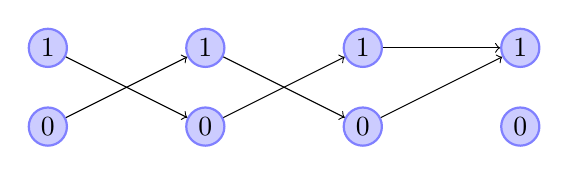
\begin{tikzpicture}
  [state/.style={circle, draw=blue!50, fill=blue!20, thick, inner sep=2pt}]
  \foreach \x in {0, 2, 4, 6}{
    \node (n1\x) at (\x, 1) [state] {1};
    \node (n0\x) at (\x, 0) [state] {0};
  }
  \draw [->] (n10) to (n02);
  \draw [->] (n00) to (n12);
  \draw [->] (n12) to (n04);
  \draw [->] (n02) to (n14);
  \draw [->] (n14) to (n16);
  \draw [->] (n04) to (n16);
\end{tikzpicture}
\end{center}

\paragraph{Coupling From The Past with no Memory}
It is quite nature to implement the CFTP sampler without \textbf{reuse}, but unfortunately, this variation of CFTP is wrong.
This sampler covers all the cases, but it does not follow the right distribution.
The probobility of this sampler returns sample $s$ equals:
\begin{align*}
&\sum_{T=1}^\infty \Pr[\mbox{$f$ has constant $s$ $|$ $\substack{\mbox{$f$ is a constant function in $T$}\\ \mbox{$\land$ $f$ is not a constant function in $\{1, \cdots, T-1\}$}}$}] \\
                  &= \sum_{T=1}^\infty \Pr[\mbox{$f$ has constant $s$ $|$ sampler halts in $T$ steps}] \Pr[\mbox{sampler halts in $T$ steps}] \\
  &= \sum_{T=1}^\infty \frac{\Pr[\mbox{constant function in $T$ steps with constant $s$}]}{\Pr[\mbox{function in $T$ steps}]} \prod_{t=1}^{T-1}\frac{\Pr[\mbox{$t$ steps not constant function}]}{\Pr[\mbox{function in $t$ steps}]} \\
\end{align*}
Actually, its hard to find any relationship between this distribution and the correct distribution.
When $s = 1$, then using the example above, we have
\begin{align*}
  \Pr[s = 1] &\geq \textcolor{red}{\Pr[\mbox{1 step}]}\textcolor{blue}{\Pr[\mbox{$f$ has constant $1$} | \mbox{1 step}]} + \textcolor{cyan}{\Pr[\mbox{2 steps}]}\textcolor{blue!50}{\Pr[\mbox{$f$ has constant $1$} | \mbox{2 steps}]} \\
             &= \textcolor{red}{\frac{1}{2}}\cdot \textcolor{blue}{1} + \textcolor{cyan}{\frac{1}{2}\cdot\frac{3}{4}}\cdot\textcolor{blue!50}{\frac{2}{3}} \\
  &= \frac{3}{4} > \frac{2}{3}
\end{align*}
So, its easy to see that this sampler does not catch the right distribution.

\begin{center}
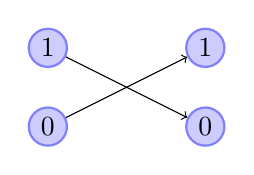
\begin{tikzpicture}
  [state/.style={circle, draw=blue!50, fill=blue!20, thick, inner sep=2pt}]
  \foreach \x in {0, 2}{
    \node (n1\x) at (\x, 1) [state] {1};
    \node (n0\x) at (\x, 0) [state] {0};
  }
  \draw [->] (n10) to (n02);
  \draw [->] (n00) to (n12);
\end{tikzpicture} \hspace{0.5cm}
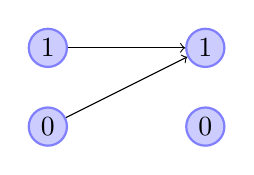
\begin{tikzpicture}
  [state/.style={circle, draw=blue!50, fill=blue!20, thick, inner sep=2pt}]
  \foreach \x in {0, 2}{
    \node (n1\x) at (\x, 1) [state] {1};
    \node (n0\x) at (\x, 0) [state] {0};
  }
  \draw [->] (n10) to (n12);
  \draw [->] (n00) to (n12);
\end{tikzpicture}
\end{center}

\begin{center}
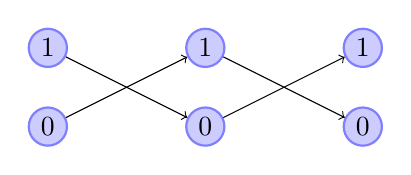
\begin{tikzpicture}
  [state/.style={circle, draw=blue!50, fill=blue!20, thick, inner sep=2pt}]
  \foreach \x in {0, 2, 4}{
    \node (n1\x) at (\x, 1) [state] {1};
    \node (n0\x) at (\x, 0) [state] {0};
  }
  \draw [->] (n10) to (n02);
  \draw [->] (n00) to (n12);
  \draw [->] (n12) to (n04);
  \draw [->] (n02) to (n14);
\end{tikzpicture} \hspace{0.5cm}
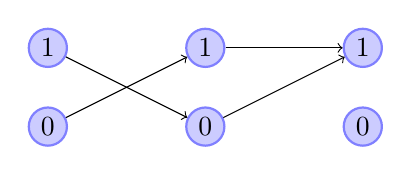
\begin{tikzpicture}
  [state/.style={circle, draw=blue!50, fill=blue!20, thick, inner sep=2pt}]
  \foreach \x in {0, 2, 4}{
    \node (n1\x) at (\x, 1) [state] {1};
    \node (n0\x) at (\x, 0) [state] {0};
  }
  \draw [->] (n10) to (n02);
  \draw [->] (n00) to (n12);
  \draw [->] (n12) to (n14);
  \draw [->] (n02) to (n14);
\end{tikzpicture} \vspace{0.5cm} \\
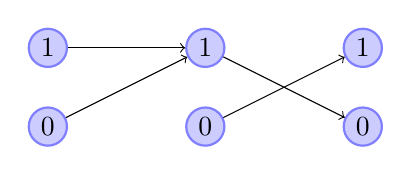
\begin{tikzpicture}
  [state/.style={circle, draw=blue!50, fill=blue!20, thick, inner sep=2pt}]
  \foreach \x in {0, 2, 4}{
    \node (n1\x) at (\x, 1) [state] {1};
    \node (n0\x) at (\x, 0) [state] {0};
  }
  \draw [->] (n10) to (n12);
  \draw [->] (n00) to (n12);
  \draw [->] (n12) to (n04);
  \draw [->] (n02) to (n14);
\end{tikzpicture} \hspace{0.5cm}
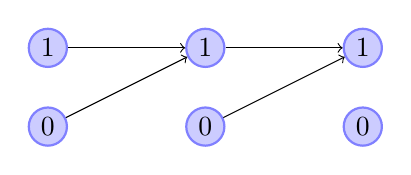
\begin{tikzpicture}
  [state/.style={circle, draw=blue!50, fill=blue!20, thick, inner sep=2pt}]
  \foreach \x in {0, 2, 4}{
    \node (n1\x) at (\x, 1) [state] {1};
    \node (n0\x) at (\x, 0) [state] {0};
  }
  \draw [->] (n10) to (n12);
  \draw [->] (n00) to (n12);
  \draw [->] (n12) to (n14);
  \draw [->] (n02) to (n14);
\end{tikzpicture} 
\end{center}
%%% Local Variables:
%%% mode: latex
%%% TeX-master: "../../notebook"
%%% End:


% understand path coupling
\section{Coupling From the Past}
\paragraph{}
Coupling from the past (CFTP) is a method with which we could perform a perfect sampling according to some distribution.
I can not find any convincing proof of this result, so I decide to prove it myself.

First, lets view Markov Chain in a new but nature way.
Suppose we have a Markov Chain $\mathcal{M}$ defined on some state set $S = \{s_1, s_2, \cdots, s_n\}$.
Note that when we execute $\mathcal{M}$, then in each turn, this chain will fix some parameters according to some distribution and move from some states to other states.
So, if we fix this random parameters, then $\mathcal{M}$ becomes a determined process, and we could view it as a function $f: S\to S$. For convenience, lets denote the determined process from time $i$ to time $i+1$ by $f_i$.
The pseudocode of CFTP is shown below.
\begin{algorithm}
  Coupling From The Past () \Begin{
    $T \gets 1$ \\
    \Repeat{$f$ becomes a constant function}{
      $f \gets f_{-T} \circ f_{-(T-1)} \circ \cdots \circ f_{-1}$ \\
      $T \gets T + 1$
    }
    \Return{$f(s_1)$}
  }
\end{algorithm}
\marginnote[-3cm]{The $\circ$ here means compose operator where $f \circ g  (x) = g(f(x))$, i.e. give $f$'s output as $g$'s input.}
\marginnote[-1.8cm]{Here, $f_{-i}$ is fixed (by random) at the first time we encountered it, and will be \textbf{reused} later.}

The idea of this sampler is quite simple.
Suppose we have a Markov Chain $\mathcal{M}$ which starts at $-\infty$ and stops at $0$, then its pretty sure that it will have the distribution $\pi$ at time $0$ (no matter which state it starts from).
Then, if we randomly determine some last finite steps of the chain (say $T$ steps), we may have the chance to recover the sample of this MC by this steps.

And, its quite easy to see that when the last $T$ steps forms a constant function we could easily recover the sample from this MC. So we have the following theorem:
\begin{theorem}
  If we have a Markov Chain $\mathcal{M}$ such that
  \[\lim_{t\to\infty} \Pr [f_0 \circ f_1 \circ \cdots \circ f_t \mbox{ is a constant function}] = 1\]
  where $f_0, f_1, \cdots, f_t$ are fixed randomly according to the transition matrix $P$ of $\mathcal{M}$,
  then the CFTP of $\mathcal{M}$ halt in finite time with probability $1$ and returns a sample according to $\pi$.
\end{theorem}
\begin{proof}
  Note that, if our algorithm could \textbf{cover} all the cases of the last finite steps of the Markov Chain, and could \textbf{recover} the sample from all these cases, then its easy to see, this algorithm should be right.

  So, here, its quite nature to ask, what means all the cases?
  Here, a case is a suffix of the chain from $-\infty$ to $0$.
  Note that, CFTP randomly choose a $f_{-t}$ at time $-t$, so if we omit the stop condition, its should cover all the cases.
  Suppose the CFTP stops at some time $T$, which means its forms a constant function $f$ and no matter how we extend this suffix, this constant will not change, so we could pack all the suffix that end with this suffix into this suffix, since they have the same sample (while do not change the distribution of sample).
  Hence, CFTP forms a cover of all the cases.

  Since $\lim_{t\to\infty}\Pr[f_0\circ f_1\circ \cdots\circ f_t] = 1$, the Markov Chain will be a constant function with probability 1 after infinite steps. Which notes us that CFTP should halt in finite time with probability $1$.
  
  Finally, since CFTP simulates a Markov Chain which have been executed for infinite steps, so the distribution of the sample should be exactly $\pi$.
\end{proof}

\subsection{Two confusing bad variations of CFTP}
\paragraph{Coupling to the future}
Its nature for us to ask, ``why not just coupling to the future?'', since this two samplers look nearly the same.
\begin{algorithm}
  Copuling To The Future () \Begin{
    $T\gets 1$ \\
    \Repeat{$f$ becomes a constant function}{
      $f \gets f_0\circ f_1\circ \cdots \circ f_T$ \\
      $T\gets T+1$
    }
    \Return{$f(s_1)$}
  }
\end{algorithm}

The problem here is that is sampler does not cover all the cases.
First, if we omit the stop condition, then it is easy to see that this sampler covers all the cases. Similarly, this sampler want to pack some of the cases so that we could stop in finite steps. Note that, if $f$ becomes a constant function in time $T$, then $f'$ will also be a constant function in time $T+1$ and so on. But $f$ and $f'$ has different constant, so we could not pack them together (we should not use the sample of $f$ to represent the sample of $f'$).
So, there is a bias in the result distribution.

Here is a quite simple example to explain this:
Suppose we have a Markov chain with state space $[2] = \{1, 2\}$ and transition matrix
\[P = \left[
    \begin{array}{cc}
      0.5 & 0.5 \\
      1   & 0
    \end{array}
  \right]\]
Obviously, $\pi = (\pi_1, \pi_2) = (\frac{2}{3}, \frac{1}{3})$.
In this example, the \emph{coupling to the future} sampler always returns $1$ as its result.

\begin{center}
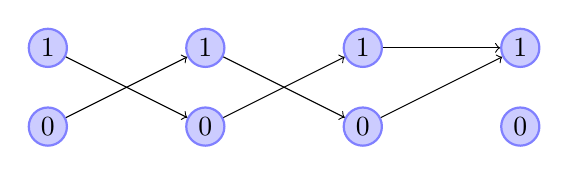
\begin{tikzpicture}
  [state/.style={circle, draw=blue!50, fill=blue!20, thick, inner sep=2pt}]
  \foreach \x in {0, 2, 4, 6}{
    \node (n1\x) at (\x, 1) [state] {1};
    \node (n0\x) at (\x, 0) [state] {0};
  }
  \draw [->] (n10) to (n02);
  \draw [->] (n00) to (n12);
  \draw [->] (n12) to (n04);
  \draw [->] (n02) to (n14);
  \draw [->] (n14) to (n16);
  \draw [->] (n04) to (n16);
\end{tikzpicture}
\end{center}

\paragraph{Coupling From The Past with no Memory}
It is quite nature to implement the CFTP sampler without \textbf{reuse}, but unfortunately, this variation of CFTP is wrong.
This sampler covers all the cases, but it does not follow the right distribution.
The probobility of this sampler returns sample $s$ equals:
\begin{align*}
&\sum_{T=1}^\infty \Pr[\mbox{$f$ has constant $s$ $|$ $\substack{\mbox{$f$ is a constant function in $T$}\\ \mbox{$\land$ $f$ is not a constant function in $\{1, \cdots, T-1\}$}}$}] \\
                  &= \sum_{T=1}^\infty \Pr[\mbox{$f$ has constant $s$ $|$ sampler halts in $T$ steps}] \Pr[\mbox{sampler halts in $T$ steps}] \\
  &= \sum_{T=1}^\infty \frac{\Pr[\mbox{constant function in $T$ steps with constant $s$}]}{\Pr[\mbox{function in $T$ steps}]} \prod_{t=1}^{T-1}\frac{\Pr[\mbox{$t$ steps not constant function}]}{\Pr[\mbox{function in $t$ steps}]} \\
\end{align*}
Actually, its hard to find any relationship between this distribution and the correct distribution.
When $s = 1$, then using the example above, we have
\begin{align*}
  \Pr[s = 1] &\geq \textcolor{red}{\Pr[\mbox{1 step}]}\textcolor{blue}{\Pr[\mbox{$f$ has constant $1$} | \mbox{1 step}]} + \textcolor{cyan}{\Pr[\mbox{2 steps}]}\textcolor{blue!50}{\Pr[\mbox{$f$ has constant $1$} | \mbox{2 steps}]} \\
             &= \textcolor{red}{\frac{1}{2}}\cdot \textcolor{blue}{1} + \textcolor{cyan}{\frac{1}{2}\cdot\frac{3}{4}}\cdot\textcolor{blue!50}{\frac{2}{3}} \\
  &= \frac{3}{4} > \frac{2}{3}
\end{align*}
So, its easy to see that this sampler does not catch the right distribution.

\begin{center}
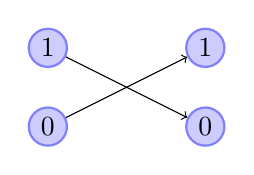
\begin{tikzpicture}
  [state/.style={circle, draw=blue!50, fill=blue!20, thick, inner sep=2pt}]
  \foreach \x in {0, 2}{
    \node (n1\x) at (\x, 1) [state] {1};
    \node (n0\x) at (\x, 0) [state] {0};
  }
  \draw [->] (n10) to (n02);
  \draw [->] (n00) to (n12);
\end{tikzpicture} \hspace{0.5cm}
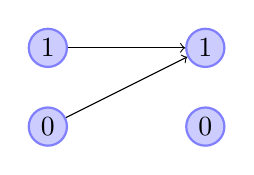
\begin{tikzpicture}
  [state/.style={circle, draw=blue!50, fill=blue!20, thick, inner sep=2pt}]
  \foreach \x in {0, 2}{
    \node (n1\x) at (\x, 1) [state] {1};
    \node (n0\x) at (\x, 0) [state] {0};
  }
  \draw [->] (n10) to (n12);
  \draw [->] (n00) to (n12);
\end{tikzpicture}
\end{center}

\begin{center}
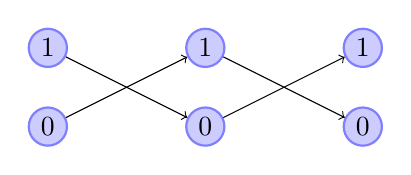
\begin{tikzpicture}
  [state/.style={circle, draw=blue!50, fill=blue!20, thick, inner sep=2pt}]
  \foreach \x in {0, 2, 4}{
    \node (n1\x) at (\x, 1) [state] {1};
    \node (n0\x) at (\x, 0) [state] {0};
  }
  \draw [->] (n10) to (n02);
  \draw [->] (n00) to (n12);
  \draw [->] (n12) to (n04);
  \draw [->] (n02) to (n14);
\end{tikzpicture} \hspace{0.5cm}
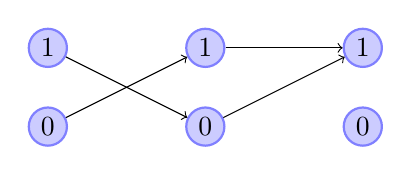
\begin{tikzpicture}
  [state/.style={circle, draw=blue!50, fill=blue!20, thick, inner sep=2pt}]
  \foreach \x in {0, 2, 4}{
    \node (n1\x) at (\x, 1) [state] {1};
    \node (n0\x) at (\x, 0) [state] {0};
  }
  \draw [->] (n10) to (n02);
  \draw [->] (n00) to (n12);
  \draw [->] (n12) to (n14);
  \draw [->] (n02) to (n14);
\end{tikzpicture} \vspace{0.5cm} \\
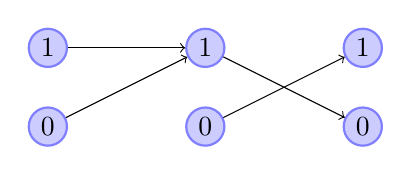
\begin{tikzpicture}
  [state/.style={circle, draw=blue!50, fill=blue!20, thick, inner sep=2pt}]
  \foreach \x in {0, 2, 4}{
    \node (n1\x) at (\x, 1) [state] {1};
    \node (n0\x) at (\x, 0) [state] {0};
  }
  \draw [->] (n10) to (n12);
  \draw [->] (n00) to (n12);
  \draw [->] (n12) to (n04);
  \draw [->] (n02) to (n14);
\end{tikzpicture} \hspace{0.5cm}
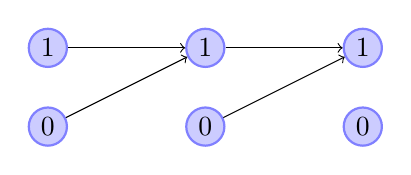
\begin{tikzpicture}
  [state/.style={circle, draw=blue!50, fill=blue!20, thick, inner sep=2pt}]
  \foreach \x in {0, 2, 4}{
    \node (n1\x) at (\x, 1) [state] {1};
    \node (n0\x) at (\x, 0) [state] {0};
  }
  \draw [->] (n10) to (n12);
  \draw [->] (n00) to (n12);
  \draw [->] (n12) to (n14);
  \draw [->] (n02) to (n14);
\end{tikzpicture} 
\end{center}
%%% Local Variables:
%%% mode: latex
%%% TeX-master: "../../notebook"
%%% End:


% understand canonical path and flow
\section{Coupling From the Past}
\paragraph{}
Coupling from the past (CFTP) is a method with which we could perform a perfect sampling according to some distribution.
I can not find any convincing proof of this result, so I decide to prove it myself.

First, lets view Markov Chain in a new but nature way.
Suppose we have a Markov Chain $\mathcal{M}$ defined on some state set $S = \{s_1, s_2, \cdots, s_n\}$.
Note that when we execute $\mathcal{M}$, then in each turn, this chain will fix some parameters according to some distribution and move from some states to other states.
So, if we fix this random parameters, then $\mathcal{M}$ becomes a determined process, and we could view it as a function $f: S\to S$. For convenience, lets denote the determined process from time $i$ to time $i+1$ by $f_i$.
The pseudocode of CFTP is shown below.
\begin{algorithm}
  Coupling From The Past () \Begin{
    $T \gets 1$ \\
    \Repeat{$f$ becomes a constant function}{
      $f \gets f_{-T} \circ f_{-(T-1)} \circ \cdots \circ f_{-1}$ \\
      $T \gets T + 1$
    }
    \Return{$f(s_1)$}
  }
\end{algorithm}
\marginnote[-3cm]{The $\circ$ here means compose operator where $f \circ g  (x) = g(f(x))$, i.e. give $f$'s output as $g$'s input.}
\marginnote[-1.8cm]{Here, $f_{-i}$ is fixed (by random) at the first time we encountered it, and will be \textbf{reused} later.}

The idea of this sampler is quite simple.
Suppose we have a Markov Chain $\mathcal{M}$ which starts at $-\infty$ and stops at $0$, then its pretty sure that it will have the distribution $\pi$ at time $0$ (no matter which state it starts from).
Then, if we randomly determine some last finite steps of the chain (say $T$ steps), we may have the chance to recover the sample of this MC by this steps.

And, its quite easy to see that when the last $T$ steps forms a constant function we could easily recover the sample from this MC. So we have the following theorem:
\begin{theorem}
  If we have a Markov Chain $\mathcal{M}$ such that
  \[\lim_{t\to\infty} \Pr [f_0 \circ f_1 \circ \cdots \circ f_t \mbox{ is a constant function}] = 1\]
  where $f_0, f_1, \cdots, f_t$ are fixed randomly according to the transition matrix $P$ of $\mathcal{M}$,
  then the CFTP of $\mathcal{M}$ halt in finite time with probability $1$ and returns a sample according to $\pi$.
\end{theorem}
\begin{proof}
  Note that, if our algorithm could \textbf{cover} all the cases of the last finite steps of the Markov Chain, and could \textbf{recover} the sample from all these cases, then its easy to see, this algorithm should be right.

  So, here, its quite nature to ask, what means all the cases?
  Here, a case is a suffix of the chain from $-\infty$ to $0$.
  Note that, CFTP randomly choose a $f_{-t}$ at time $-t$, so if we omit the stop condition, its should cover all the cases.
  Suppose the CFTP stops at some time $T$, which means its forms a constant function $f$ and no matter how we extend this suffix, this constant will not change, so we could pack all the suffix that end with this suffix into this suffix, since they have the same sample (while do not change the distribution of sample).
  Hence, CFTP forms a cover of all the cases.

  Since $\lim_{t\to\infty}\Pr[f_0\circ f_1\circ \cdots\circ f_t] = 1$, the Markov Chain will be a constant function with probability 1 after infinite steps. Which notes us that CFTP should halt in finite time with probability $1$.
  
  Finally, since CFTP simulates a Markov Chain which have been executed for infinite steps, so the distribution of the sample should be exactly $\pi$.
\end{proof}

\subsection{Two confusing bad variations of CFTP}
\paragraph{Coupling to the future}
Its nature for us to ask, ``why not just coupling to the future?'', since this two samplers look nearly the same.
\begin{algorithm}
  Copuling To The Future () \Begin{
    $T\gets 1$ \\
    \Repeat{$f$ becomes a constant function}{
      $f \gets f_0\circ f_1\circ \cdots \circ f_T$ \\
      $T\gets T+1$
    }
    \Return{$f(s_1)$}
  }
\end{algorithm}

The problem here is that is sampler does not cover all the cases.
First, if we omit the stop condition, then it is easy to see that this sampler covers all the cases. Similarly, this sampler want to pack some of the cases so that we could stop in finite steps. Note that, if $f$ becomes a constant function in time $T$, then $f'$ will also be a constant function in time $T+1$ and so on. But $f$ and $f'$ has different constant, so we could not pack them together (we should not use the sample of $f$ to represent the sample of $f'$).
So, there is a bias in the result distribution.

Here is a quite simple example to explain this:
Suppose we have a Markov chain with state space $[2] = \{1, 2\}$ and transition matrix
\[P = \left[
    \begin{array}{cc}
      0.5 & 0.5 \\
      1   & 0
    \end{array}
  \right]\]
Obviously, $\pi = (\pi_1, \pi_2) = (\frac{2}{3}, \frac{1}{3})$.
In this example, the \emph{coupling to the future} sampler always returns $1$ as its result.

\begin{center}
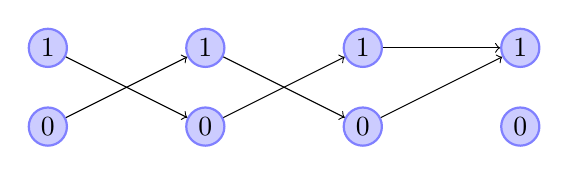
\begin{tikzpicture}
  [state/.style={circle, draw=blue!50, fill=blue!20, thick, inner sep=2pt}]
  \foreach \x in {0, 2, 4, 6}{
    \node (n1\x) at (\x, 1) [state] {1};
    \node (n0\x) at (\x, 0) [state] {0};
  }
  \draw [->] (n10) to (n02);
  \draw [->] (n00) to (n12);
  \draw [->] (n12) to (n04);
  \draw [->] (n02) to (n14);
  \draw [->] (n14) to (n16);
  \draw [->] (n04) to (n16);
\end{tikzpicture}
\end{center}

\paragraph{Coupling From The Past with no Memory}
It is quite nature to implement the CFTP sampler without \textbf{reuse}, but unfortunately, this variation of CFTP is wrong.
This sampler covers all the cases, but it does not follow the right distribution.
The probobility of this sampler returns sample $s$ equals:
\begin{align*}
&\sum_{T=1}^\infty \Pr[\mbox{$f$ has constant $s$ $|$ $\substack{\mbox{$f$ is a constant function in $T$}\\ \mbox{$\land$ $f$ is not a constant function in $\{1, \cdots, T-1\}$}}$}] \\
                  &= \sum_{T=1}^\infty \Pr[\mbox{$f$ has constant $s$ $|$ sampler halts in $T$ steps}] \Pr[\mbox{sampler halts in $T$ steps}] \\
  &= \sum_{T=1}^\infty \frac{\Pr[\mbox{constant function in $T$ steps with constant $s$}]}{\Pr[\mbox{function in $T$ steps}]} \prod_{t=1}^{T-1}\frac{\Pr[\mbox{$t$ steps not constant function}]}{\Pr[\mbox{function in $t$ steps}]} \\
\end{align*}
Actually, its hard to find any relationship between this distribution and the correct distribution.
When $s = 1$, then using the example above, we have
\begin{align*}
  \Pr[s = 1] &\geq \textcolor{red}{\Pr[\mbox{1 step}]}\textcolor{blue}{\Pr[\mbox{$f$ has constant $1$} | \mbox{1 step}]} + \textcolor{cyan}{\Pr[\mbox{2 steps}]}\textcolor{blue!50}{\Pr[\mbox{$f$ has constant $1$} | \mbox{2 steps}]} \\
             &= \textcolor{red}{\frac{1}{2}}\cdot \textcolor{blue}{1} + \textcolor{cyan}{\frac{1}{2}\cdot\frac{3}{4}}\cdot\textcolor{blue!50}{\frac{2}{3}} \\
  &= \frac{3}{4} > \frac{2}{3}
\end{align*}
So, its easy to see that this sampler does not catch the right distribution.

\begin{center}
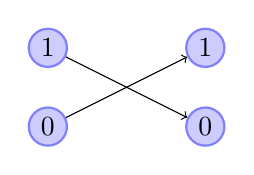
\begin{tikzpicture}
  [state/.style={circle, draw=blue!50, fill=blue!20, thick, inner sep=2pt}]
  \foreach \x in {0, 2}{
    \node (n1\x) at (\x, 1) [state] {1};
    \node (n0\x) at (\x, 0) [state] {0};
  }
  \draw [->] (n10) to (n02);
  \draw [->] (n00) to (n12);
\end{tikzpicture} \hspace{0.5cm}
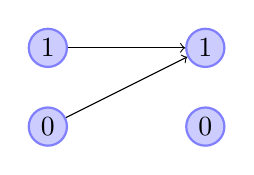
\begin{tikzpicture}
  [state/.style={circle, draw=blue!50, fill=blue!20, thick, inner sep=2pt}]
  \foreach \x in {0, 2}{
    \node (n1\x) at (\x, 1) [state] {1};
    \node (n0\x) at (\x, 0) [state] {0};
  }
  \draw [->] (n10) to (n12);
  \draw [->] (n00) to (n12);
\end{tikzpicture}
\end{center}

\begin{center}
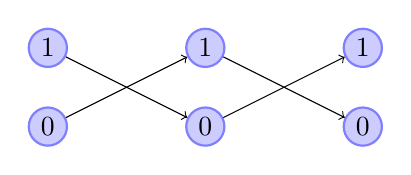
\begin{tikzpicture}
  [state/.style={circle, draw=blue!50, fill=blue!20, thick, inner sep=2pt}]
  \foreach \x in {0, 2, 4}{
    \node (n1\x) at (\x, 1) [state] {1};
    \node (n0\x) at (\x, 0) [state] {0};
  }
  \draw [->] (n10) to (n02);
  \draw [->] (n00) to (n12);
  \draw [->] (n12) to (n04);
  \draw [->] (n02) to (n14);
\end{tikzpicture} \hspace{0.5cm}
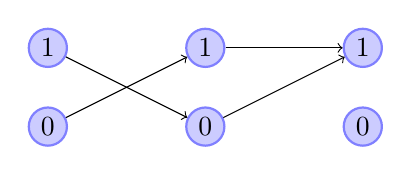
\begin{tikzpicture}
  [state/.style={circle, draw=blue!50, fill=blue!20, thick, inner sep=2pt}]
  \foreach \x in {0, 2, 4}{
    \node (n1\x) at (\x, 1) [state] {1};
    \node (n0\x) at (\x, 0) [state] {0};
  }
  \draw [->] (n10) to (n02);
  \draw [->] (n00) to (n12);
  \draw [->] (n12) to (n14);
  \draw [->] (n02) to (n14);
\end{tikzpicture} \vspace{0.5cm} \\
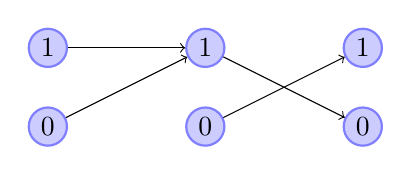
\begin{tikzpicture}
  [state/.style={circle, draw=blue!50, fill=blue!20, thick, inner sep=2pt}]
  \foreach \x in {0, 2, 4}{
    \node (n1\x) at (\x, 1) [state] {1};
    \node (n0\x) at (\x, 0) [state] {0};
  }
  \draw [->] (n10) to (n12);
  \draw [->] (n00) to (n12);
  \draw [->] (n12) to (n04);
  \draw [->] (n02) to (n14);
\end{tikzpicture} \hspace{0.5cm}
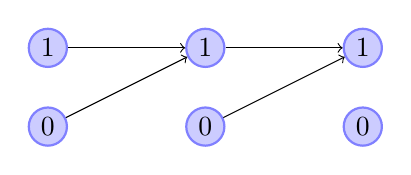
\begin{tikzpicture}
  [state/.style={circle, draw=blue!50, fill=blue!20, thick, inner sep=2pt}]
  \foreach \x in {0, 2, 4}{
    \node (n1\x) at (\x, 1) [state] {1};
    \node (n0\x) at (\x, 0) [state] {0};
  }
  \draw [->] (n10) to (n12);
  \draw [->] (n00) to (n12);
  \draw [->] (n12) to (n14);
  \draw [->] (n02) to (n14);
\end{tikzpicture} 
\end{center}
%%% Local Variables:
%%% mode: latex
%%% TeX-master: "../../notebook"
%%% End:


% the lower bound for mixing time
\section{Coupling From the Past}
\paragraph{}
Coupling from the past (CFTP) is a method with which we could perform a perfect sampling according to some distribution.
I can not find any convincing proof of this result, so I decide to prove it myself.

First, lets view Markov Chain in a new but nature way.
Suppose we have a Markov Chain $\mathcal{M}$ defined on some state set $S = \{s_1, s_2, \cdots, s_n\}$.
Note that when we execute $\mathcal{M}$, then in each turn, this chain will fix some parameters according to some distribution and move from some states to other states.
So, if we fix this random parameters, then $\mathcal{M}$ becomes a determined process, and we could view it as a function $f: S\to S$. For convenience, lets denote the determined process from time $i$ to time $i+1$ by $f_i$.
The pseudocode of CFTP is shown below.
\begin{algorithm}
  Coupling From The Past () \Begin{
    $T \gets 1$ \\
    \Repeat{$f$ becomes a constant function}{
      $f \gets f_{-T} \circ f_{-(T-1)} \circ \cdots \circ f_{-1}$ \\
      $T \gets T + 1$
    }
    \Return{$f(s_1)$}
  }
\end{algorithm}
\marginnote[-3cm]{The $\circ$ here means compose operator where $f \circ g  (x) = g(f(x))$, i.e. give $f$'s output as $g$'s input.}
\marginnote[-1.8cm]{Here, $f_{-i}$ is fixed (by random) at the first time we encountered it, and will be \textbf{reused} later.}

The idea of this sampler is quite simple.
Suppose we have a Markov Chain $\mathcal{M}$ which starts at $-\infty$ and stops at $0$, then its pretty sure that it will have the distribution $\pi$ at time $0$ (no matter which state it starts from).
Then, if we randomly determine some last finite steps of the chain (say $T$ steps), we may have the chance to recover the sample of this MC by this steps.

And, its quite easy to see that when the last $T$ steps forms a constant function we could easily recover the sample from this MC. So we have the following theorem:
\begin{theorem}
  If we have a Markov Chain $\mathcal{M}$ such that
  \[\lim_{t\to\infty} \Pr [f_0 \circ f_1 \circ \cdots \circ f_t \mbox{ is a constant function}] = 1\]
  where $f_0, f_1, \cdots, f_t$ are fixed randomly according to the transition matrix $P$ of $\mathcal{M}$,
  then the CFTP of $\mathcal{M}$ halt in finite time with probability $1$ and returns a sample according to $\pi$.
\end{theorem}
\begin{proof}
  Note that, if our algorithm could \textbf{cover} all the cases of the last finite steps of the Markov Chain, and could \textbf{recover} the sample from all these cases, then its easy to see, this algorithm should be right.

  So, here, its quite nature to ask, what means all the cases?
  Here, a case is a suffix of the chain from $-\infty$ to $0$.
  Note that, CFTP randomly choose a $f_{-t}$ at time $-t$, so if we omit the stop condition, its should cover all the cases.
  Suppose the CFTP stops at some time $T$, which means its forms a constant function $f$ and no matter how we extend this suffix, this constant will not change, so we could pack all the suffix that end with this suffix into this suffix, since they have the same sample (while do not change the distribution of sample).
  Hence, CFTP forms a cover of all the cases.

  Since $\lim_{t\to\infty}\Pr[f_0\circ f_1\circ \cdots\circ f_t] = 1$, the Markov Chain will be a constant function with probability 1 after infinite steps. Which notes us that CFTP should halt in finite time with probability $1$.
  
  Finally, since CFTP simulates a Markov Chain which have been executed for infinite steps, so the distribution of the sample should be exactly $\pi$.
\end{proof}

\subsection{Two confusing bad variations of CFTP}
\paragraph{Coupling to the future}
Its nature for us to ask, ``why not just coupling to the future?'', since this two samplers look nearly the same.
\begin{algorithm}
  Copuling To The Future () \Begin{
    $T\gets 1$ \\
    \Repeat{$f$ becomes a constant function}{
      $f \gets f_0\circ f_1\circ \cdots \circ f_T$ \\
      $T\gets T+1$
    }
    \Return{$f(s_1)$}
  }
\end{algorithm}

The problem here is that is sampler does not cover all the cases.
First, if we omit the stop condition, then it is easy to see that this sampler covers all the cases. Similarly, this sampler want to pack some of the cases so that we could stop in finite steps. Note that, if $f$ becomes a constant function in time $T$, then $f'$ will also be a constant function in time $T+1$ and so on. But $f$ and $f'$ has different constant, so we could not pack them together (we should not use the sample of $f$ to represent the sample of $f'$).
So, there is a bias in the result distribution.

Here is a quite simple example to explain this:
Suppose we have a Markov chain with state space $[2] = \{1, 2\}$ and transition matrix
\[P = \left[
    \begin{array}{cc}
      0.5 & 0.5 \\
      1   & 0
    \end{array}
  \right]\]
Obviously, $\pi = (\pi_1, \pi_2) = (\frac{2}{3}, \frac{1}{3})$.
In this example, the \emph{coupling to the future} sampler always returns $1$ as its result.

\begin{center}
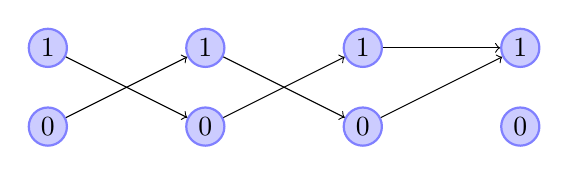
\begin{tikzpicture}
  [state/.style={circle, draw=blue!50, fill=blue!20, thick, inner sep=2pt}]
  \foreach \x in {0, 2, 4, 6}{
    \node (n1\x) at (\x, 1) [state] {1};
    \node (n0\x) at (\x, 0) [state] {0};
  }
  \draw [->] (n10) to (n02);
  \draw [->] (n00) to (n12);
  \draw [->] (n12) to (n04);
  \draw [->] (n02) to (n14);
  \draw [->] (n14) to (n16);
  \draw [->] (n04) to (n16);
\end{tikzpicture}
\end{center}

\paragraph{Coupling From The Past with no Memory}
It is quite nature to implement the CFTP sampler without \textbf{reuse}, but unfortunately, this variation of CFTP is wrong.
This sampler covers all the cases, but it does not follow the right distribution.
The probobility of this sampler returns sample $s$ equals:
\begin{align*}
&\sum_{T=1}^\infty \Pr[\mbox{$f$ has constant $s$ $|$ $\substack{\mbox{$f$ is a constant function in $T$}\\ \mbox{$\land$ $f$ is not a constant function in $\{1, \cdots, T-1\}$}}$}] \\
                  &= \sum_{T=1}^\infty \Pr[\mbox{$f$ has constant $s$ $|$ sampler halts in $T$ steps}] \Pr[\mbox{sampler halts in $T$ steps}] \\
  &= \sum_{T=1}^\infty \frac{\Pr[\mbox{constant function in $T$ steps with constant $s$}]}{\Pr[\mbox{function in $T$ steps}]} \prod_{t=1}^{T-1}\frac{\Pr[\mbox{$t$ steps not constant function}]}{\Pr[\mbox{function in $t$ steps}]} \\
\end{align*}
Actually, its hard to find any relationship between this distribution and the correct distribution.
When $s = 1$, then using the example above, we have
\begin{align*}
  \Pr[s = 1] &\geq \textcolor{red}{\Pr[\mbox{1 step}]}\textcolor{blue}{\Pr[\mbox{$f$ has constant $1$} | \mbox{1 step}]} + \textcolor{cyan}{\Pr[\mbox{2 steps}]}\textcolor{blue!50}{\Pr[\mbox{$f$ has constant $1$} | \mbox{2 steps}]} \\
             &= \textcolor{red}{\frac{1}{2}}\cdot \textcolor{blue}{1} + \textcolor{cyan}{\frac{1}{2}\cdot\frac{3}{4}}\cdot\textcolor{blue!50}{\frac{2}{3}} \\
  &= \frac{3}{4} > \frac{2}{3}
\end{align*}
So, its easy to see that this sampler does not catch the right distribution.

\begin{center}
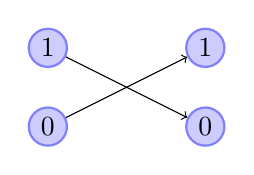
\begin{tikzpicture}
  [state/.style={circle, draw=blue!50, fill=blue!20, thick, inner sep=2pt}]
  \foreach \x in {0, 2}{
    \node (n1\x) at (\x, 1) [state] {1};
    \node (n0\x) at (\x, 0) [state] {0};
  }
  \draw [->] (n10) to (n02);
  \draw [->] (n00) to (n12);
\end{tikzpicture} \hspace{0.5cm}
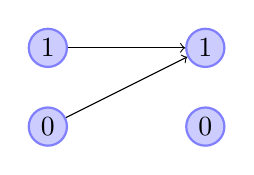
\begin{tikzpicture}
  [state/.style={circle, draw=blue!50, fill=blue!20, thick, inner sep=2pt}]
  \foreach \x in {0, 2}{
    \node (n1\x) at (\x, 1) [state] {1};
    \node (n0\x) at (\x, 0) [state] {0};
  }
  \draw [->] (n10) to (n12);
  \draw [->] (n00) to (n12);
\end{tikzpicture}
\end{center}

\begin{center}
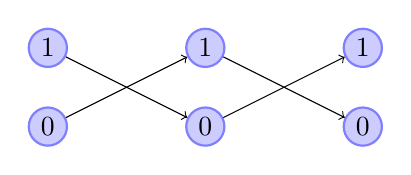
\begin{tikzpicture}
  [state/.style={circle, draw=blue!50, fill=blue!20, thick, inner sep=2pt}]
  \foreach \x in {0, 2, 4}{
    \node (n1\x) at (\x, 1) [state] {1};
    \node (n0\x) at (\x, 0) [state] {0};
  }
  \draw [->] (n10) to (n02);
  \draw [->] (n00) to (n12);
  \draw [->] (n12) to (n04);
  \draw [->] (n02) to (n14);
\end{tikzpicture} \hspace{0.5cm}
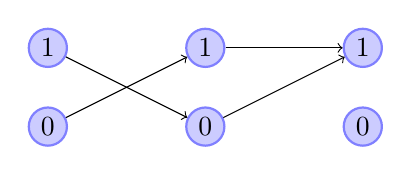
\begin{tikzpicture}
  [state/.style={circle, draw=blue!50, fill=blue!20, thick, inner sep=2pt}]
  \foreach \x in {0, 2, 4}{
    \node (n1\x) at (\x, 1) [state] {1};
    \node (n0\x) at (\x, 0) [state] {0};
  }
  \draw [->] (n10) to (n02);
  \draw [->] (n00) to (n12);
  \draw [->] (n12) to (n14);
  \draw [->] (n02) to (n14);
\end{tikzpicture} \vspace{0.5cm} \\
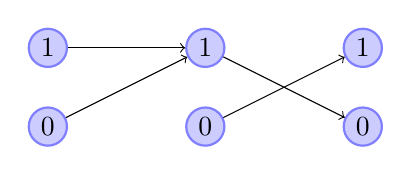
\begin{tikzpicture}
  [state/.style={circle, draw=blue!50, fill=blue!20, thick, inner sep=2pt}]
  \foreach \x in {0, 2, 4}{
    \node (n1\x) at (\x, 1) [state] {1};
    \node (n0\x) at (\x, 0) [state] {0};
  }
  \draw [->] (n10) to (n12);
  \draw [->] (n00) to (n12);
  \draw [->] (n12) to (n04);
  \draw [->] (n02) to (n14);
\end{tikzpicture} \hspace{0.5cm}
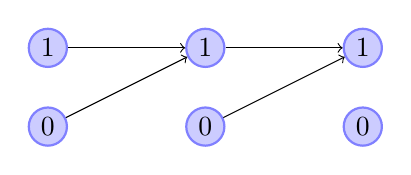
\begin{tikzpicture}
  [state/.style={circle, draw=blue!50, fill=blue!20, thick, inner sep=2pt}]
  \foreach \x in {0, 2, 4}{
    \node (n1\x) at (\x, 1) [state] {1};
    \node (n0\x) at (\x, 0) [state] {0};
  }
  \draw [->] (n10) to (n12);
  \draw [->] (n00) to (n12);
  \draw [->] (n12) to (n14);
  \draw [->] (n02) to (n14);
\end{tikzpicture} 
\end{center}
%%% Local Variables:
%%% mode: latex
%%% TeX-master: "../../notebook"
%%% End:


\chapter{Topics Related to Probability}
\clearpage

% definition for expectation and conditional expectation
\section{Coupling From the Past}
\paragraph{}
Coupling from the past (CFTP) is a method with which we could perform a perfect sampling according to some distribution.
I can not find any convincing proof of this result, so I decide to prove it myself.

First, lets view Markov Chain in a new but nature way.
Suppose we have a Markov Chain $\mathcal{M}$ defined on some state set $S = \{s_1, s_2, \cdots, s_n\}$.
Note that when we execute $\mathcal{M}$, then in each turn, this chain will fix some parameters according to some distribution and move from some states to other states.
So, if we fix this random parameters, then $\mathcal{M}$ becomes a determined process, and we could view it as a function $f: S\to S$. For convenience, lets denote the determined process from time $i$ to time $i+1$ by $f_i$.
The pseudocode of CFTP is shown below.
\begin{algorithm}
  Coupling From The Past () \Begin{
    $T \gets 1$ \\
    \Repeat{$f$ becomes a constant function}{
      $f \gets f_{-T} \circ f_{-(T-1)} \circ \cdots \circ f_{-1}$ \\
      $T \gets T + 1$
    }
    \Return{$f(s_1)$}
  }
\end{algorithm}
\marginnote[-3cm]{The $\circ$ here means compose operator where $f \circ g  (x) = g(f(x))$, i.e. give $f$'s output as $g$'s input.}
\marginnote[-1.8cm]{Here, $f_{-i}$ is fixed (by random) at the first time we encountered it, and will be \textbf{reused} later.}

The idea of this sampler is quite simple.
Suppose we have a Markov Chain $\mathcal{M}$ which starts at $-\infty$ and stops at $0$, then its pretty sure that it will have the distribution $\pi$ at time $0$ (no matter which state it starts from).
Then, if we randomly determine some last finite steps of the chain (say $T$ steps), we may have the chance to recover the sample of this MC by this steps.

And, its quite easy to see that when the last $T$ steps forms a constant function we could easily recover the sample from this MC. So we have the following theorem:
\begin{theorem}
  If we have a Markov Chain $\mathcal{M}$ such that
  \[\lim_{t\to\infty} \Pr [f_0 \circ f_1 \circ \cdots \circ f_t \mbox{ is a constant function}] = 1\]
  where $f_0, f_1, \cdots, f_t$ are fixed randomly according to the transition matrix $P$ of $\mathcal{M}$,
  then the CFTP of $\mathcal{M}$ halt in finite time with probability $1$ and returns a sample according to $\pi$.
\end{theorem}
\begin{proof}
  Note that, if our algorithm could \textbf{cover} all the cases of the last finite steps of the Markov Chain, and could \textbf{recover} the sample from all these cases, then its easy to see, this algorithm should be right.

  So, here, its quite nature to ask, what means all the cases?
  Here, a case is a suffix of the chain from $-\infty$ to $0$.
  Note that, CFTP randomly choose a $f_{-t}$ at time $-t$, so if we omit the stop condition, its should cover all the cases.
  Suppose the CFTP stops at some time $T$, which means its forms a constant function $f$ and no matter how we extend this suffix, this constant will not change, so we could pack all the suffix that end with this suffix into this suffix, since they have the same sample (while do not change the distribution of sample).
  Hence, CFTP forms a cover of all the cases.

  Since $\lim_{t\to\infty}\Pr[f_0\circ f_1\circ \cdots\circ f_t] = 1$, the Markov Chain will be a constant function with probability 1 after infinite steps. Which notes us that CFTP should halt in finite time with probability $1$.
  
  Finally, since CFTP simulates a Markov Chain which have been executed for infinite steps, so the distribution of the sample should be exactly $\pi$.
\end{proof}

\subsection{Two confusing bad variations of CFTP}
\paragraph{Coupling to the future}
Its nature for us to ask, ``why not just coupling to the future?'', since this two samplers look nearly the same.
\begin{algorithm}
  Copuling To The Future () \Begin{
    $T\gets 1$ \\
    \Repeat{$f$ becomes a constant function}{
      $f \gets f_0\circ f_1\circ \cdots \circ f_T$ \\
      $T\gets T+1$
    }
    \Return{$f(s_1)$}
  }
\end{algorithm}

The problem here is that is sampler does not cover all the cases.
First, if we omit the stop condition, then it is easy to see that this sampler covers all the cases. Similarly, this sampler want to pack some of the cases so that we could stop in finite steps. Note that, if $f$ becomes a constant function in time $T$, then $f'$ will also be a constant function in time $T+1$ and so on. But $f$ and $f'$ has different constant, so we could not pack them together (we should not use the sample of $f$ to represent the sample of $f'$).
So, there is a bias in the result distribution.

Here is a quite simple example to explain this:
Suppose we have a Markov chain with state space $[2] = \{1, 2\}$ and transition matrix
\[P = \left[
    \begin{array}{cc}
      0.5 & 0.5 \\
      1   & 0
    \end{array}
  \right]\]
Obviously, $\pi = (\pi_1, \pi_2) = (\frac{2}{3}, \frac{1}{3})$.
In this example, the \emph{coupling to the future} sampler always returns $1$ as its result.

\begin{center}
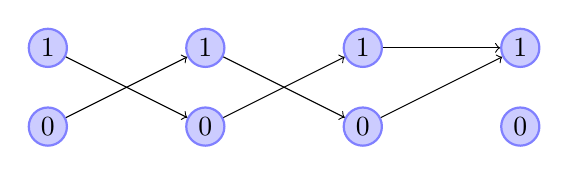
\begin{tikzpicture}
  [state/.style={circle, draw=blue!50, fill=blue!20, thick, inner sep=2pt}]
  \foreach \x in {0, 2, 4, 6}{
    \node (n1\x) at (\x, 1) [state] {1};
    \node (n0\x) at (\x, 0) [state] {0};
  }
  \draw [->] (n10) to (n02);
  \draw [->] (n00) to (n12);
  \draw [->] (n12) to (n04);
  \draw [->] (n02) to (n14);
  \draw [->] (n14) to (n16);
  \draw [->] (n04) to (n16);
\end{tikzpicture}
\end{center}

\paragraph{Coupling From The Past with no Memory}
It is quite nature to implement the CFTP sampler without \textbf{reuse}, but unfortunately, this variation of CFTP is wrong.
This sampler covers all the cases, but it does not follow the right distribution.
The probobility of this sampler returns sample $s$ equals:
\begin{align*}
&\sum_{T=1}^\infty \Pr[\mbox{$f$ has constant $s$ $|$ $\substack{\mbox{$f$ is a constant function in $T$}\\ \mbox{$\land$ $f$ is not a constant function in $\{1, \cdots, T-1\}$}}$}] \\
                  &= \sum_{T=1}^\infty \Pr[\mbox{$f$ has constant $s$ $|$ sampler halts in $T$ steps}] \Pr[\mbox{sampler halts in $T$ steps}] \\
  &= \sum_{T=1}^\infty \frac{\Pr[\mbox{constant function in $T$ steps with constant $s$}]}{\Pr[\mbox{function in $T$ steps}]} \prod_{t=1}^{T-1}\frac{\Pr[\mbox{$t$ steps not constant function}]}{\Pr[\mbox{function in $t$ steps}]} \\
\end{align*}
Actually, its hard to find any relationship between this distribution and the correct distribution.
When $s = 1$, then using the example above, we have
\begin{align*}
  \Pr[s = 1] &\geq \textcolor{red}{\Pr[\mbox{1 step}]}\textcolor{blue}{\Pr[\mbox{$f$ has constant $1$} | \mbox{1 step}]} + \textcolor{cyan}{\Pr[\mbox{2 steps}]}\textcolor{blue!50}{\Pr[\mbox{$f$ has constant $1$} | \mbox{2 steps}]} \\
             &= \textcolor{red}{\frac{1}{2}}\cdot \textcolor{blue}{1} + \textcolor{cyan}{\frac{1}{2}\cdot\frac{3}{4}}\cdot\textcolor{blue!50}{\frac{2}{3}} \\
  &= \frac{3}{4} > \frac{2}{3}
\end{align*}
So, its easy to see that this sampler does not catch the right distribution.

\begin{center}
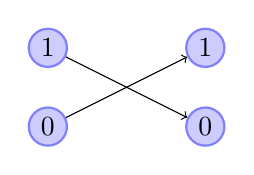
\begin{tikzpicture}
  [state/.style={circle, draw=blue!50, fill=blue!20, thick, inner sep=2pt}]
  \foreach \x in {0, 2}{
    \node (n1\x) at (\x, 1) [state] {1};
    \node (n0\x) at (\x, 0) [state] {0};
  }
  \draw [->] (n10) to (n02);
  \draw [->] (n00) to (n12);
\end{tikzpicture} \hspace{0.5cm}
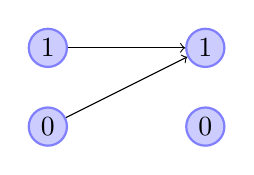
\begin{tikzpicture}
  [state/.style={circle, draw=blue!50, fill=blue!20, thick, inner sep=2pt}]
  \foreach \x in {0, 2}{
    \node (n1\x) at (\x, 1) [state] {1};
    \node (n0\x) at (\x, 0) [state] {0};
  }
  \draw [->] (n10) to (n12);
  \draw [->] (n00) to (n12);
\end{tikzpicture}
\end{center}

\begin{center}
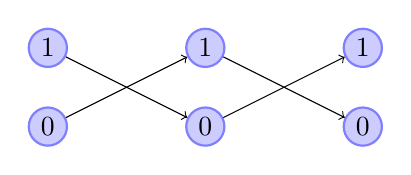
\begin{tikzpicture}
  [state/.style={circle, draw=blue!50, fill=blue!20, thick, inner sep=2pt}]
  \foreach \x in {0, 2, 4}{
    \node (n1\x) at (\x, 1) [state] {1};
    \node (n0\x) at (\x, 0) [state] {0};
  }
  \draw [->] (n10) to (n02);
  \draw [->] (n00) to (n12);
  \draw [->] (n12) to (n04);
  \draw [->] (n02) to (n14);
\end{tikzpicture} \hspace{0.5cm}
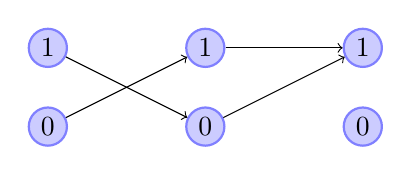
\begin{tikzpicture}
  [state/.style={circle, draw=blue!50, fill=blue!20, thick, inner sep=2pt}]
  \foreach \x in {0, 2, 4}{
    \node (n1\x) at (\x, 1) [state] {1};
    \node (n0\x) at (\x, 0) [state] {0};
  }
  \draw [->] (n10) to (n02);
  \draw [->] (n00) to (n12);
  \draw [->] (n12) to (n14);
  \draw [->] (n02) to (n14);
\end{tikzpicture} \vspace{0.5cm} \\
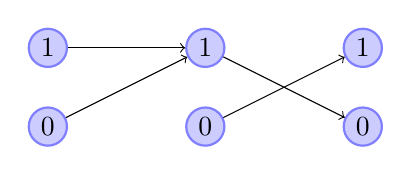
\begin{tikzpicture}
  [state/.style={circle, draw=blue!50, fill=blue!20, thick, inner sep=2pt}]
  \foreach \x in {0, 2, 4}{
    \node (n1\x) at (\x, 1) [state] {1};
    \node (n0\x) at (\x, 0) [state] {0};
  }
  \draw [->] (n10) to (n12);
  \draw [->] (n00) to (n12);
  \draw [->] (n12) to (n04);
  \draw [->] (n02) to (n14);
\end{tikzpicture} \hspace{0.5cm}
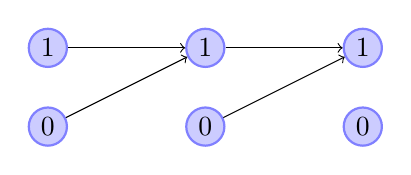
\begin{tikzpicture}
  [state/.style={circle, draw=blue!50, fill=blue!20, thick, inner sep=2pt}]
  \foreach \x in {0, 2, 4}{
    \node (n1\x) at (\x, 1) [state] {1};
    \node (n0\x) at (\x, 0) [state] {0};
  }
  \draw [->] (n10) to (n12);
  \draw [->] (n00) to (n12);
  \draw [->] (n12) to (n14);
  \draw [->] (n02) to (n14);
\end{tikzpicture} 
\end{center}
%%% Local Variables:
%%% mode: latex
%%% TeX-master: "../../notebook"
%%% End:


% some useful properties for expectation and variance
\section{Coupling From the Past}
\paragraph{}
Coupling from the past (CFTP) is a method with which we could perform a perfect sampling according to some distribution.
I can not find any convincing proof of this result, so I decide to prove it myself.

First, lets view Markov Chain in a new but nature way.
Suppose we have a Markov Chain $\mathcal{M}$ defined on some state set $S = \{s_1, s_2, \cdots, s_n\}$.
Note that when we execute $\mathcal{M}$, then in each turn, this chain will fix some parameters according to some distribution and move from some states to other states.
So, if we fix this random parameters, then $\mathcal{M}$ becomes a determined process, and we could view it as a function $f: S\to S$. For convenience, lets denote the determined process from time $i$ to time $i+1$ by $f_i$.
The pseudocode of CFTP is shown below.
\begin{algorithm}
  Coupling From The Past () \Begin{
    $T \gets 1$ \\
    \Repeat{$f$ becomes a constant function}{
      $f \gets f_{-T} \circ f_{-(T-1)} \circ \cdots \circ f_{-1}$ \\
      $T \gets T + 1$
    }
    \Return{$f(s_1)$}
  }
\end{algorithm}
\marginnote[-3cm]{The $\circ$ here means compose operator where $f \circ g  (x) = g(f(x))$, i.e. give $f$'s output as $g$'s input.}
\marginnote[-1.8cm]{Here, $f_{-i}$ is fixed (by random) at the first time we encountered it, and will be \textbf{reused} later.}

The idea of this sampler is quite simple.
Suppose we have a Markov Chain $\mathcal{M}$ which starts at $-\infty$ and stops at $0$, then its pretty sure that it will have the distribution $\pi$ at time $0$ (no matter which state it starts from).
Then, if we randomly determine some last finite steps of the chain (say $T$ steps), we may have the chance to recover the sample of this MC by this steps.

And, its quite easy to see that when the last $T$ steps forms a constant function we could easily recover the sample from this MC. So we have the following theorem:
\begin{theorem}
  If we have a Markov Chain $\mathcal{M}$ such that
  \[\lim_{t\to\infty} \Pr [f_0 \circ f_1 \circ \cdots \circ f_t \mbox{ is a constant function}] = 1\]
  where $f_0, f_1, \cdots, f_t$ are fixed randomly according to the transition matrix $P$ of $\mathcal{M}$,
  then the CFTP of $\mathcal{M}$ halt in finite time with probability $1$ and returns a sample according to $\pi$.
\end{theorem}
\begin{proof}
  Note that, if our algorithm could \textbf{cover} all the cases of the last finite steps of the Markov Chain, and could \textbf{recover} the sample from all these cases, then its easy to see, this algorithm should be right.

  So, here, its quite nature to ask, what means all the cases?
  Here, a case is a suffix of the chain from $-\infty$ to $0$.
  Note that, CFTP randomly choose a $f_{-t}$ at time $-t$, so if we omit the stop condition, its should cover all the cases.
  Suppose the CFTP stops at some time $T$, which means its forms a constant function $f$ and no matter how we extend this suffix, this constant will not change, so we could pack all the suffix that end with this suffix into this suffix, since they have the same sample (while do not change the distribution of sample).
  Hence, CFTP forms a cover of all the cases.

  Since $\lim_{t\to\infty}\Pr[f_0\circ f_1\circ \cdots\circ f_t] = 1$, the Markov Chain will be a constant function with probability 1 after infinite steps. Which notes us that CFTP should halt in finite time with probability $1$.
  
  Finally, since CFTP simulates a Markov Chain which have been executed for infinite steps, so the distribution of the sample should be exactly $\pi$.
\end{proof}

\subsection{Two confusing bad variations of CFTP}
\paragraph{Coupling to the future}
Its nature for us to ask, ``why not just coupling to the future?'', since this two samplers look nearly the same.
\begin{algorithm}
  Copuling To The Future () \Begin{
    $T\gets 1$ \\
    \Repeat{$f$ becomes a constant function}{
      $f \gets f_0\circ f_1\circ \cdots \circ f_T$ \\
      $T\gets T+1$
    }
    \Return{$f(s_1)$}
  }
\end{algorithm}

The problem here is that is sampler does not cover all the cases.
First, if we omit the stop condition, then it is easy to see that this sampler covers all the cases. Similarly, this sampler want to pack some of the cases so that we could stop in finite steps. Note that, if $f$ becomes a constant function in time $T$, then $f'$ will also be a constant function in time $T+1$ and so on. But $f$ and $f'$ has different constant, so we could not pack them together (we should not use the sample of $f$ to represent the sample of $f'$).
So, there is a bias in the result distribution.

Here is a quite simple example to explain this:
Suppose we have a Markov chain with state space $[2] = \{1, 2\}$ and transition matrix
\[P = \left[
    \begin{array}{cc}
      0.5 & 0.5 \\
      1   & 0
    \end{array}
  \right]\]
Obviously, $\pi = (\pi_1, \pi_2) = (\frac{2}{3}, \frac{1}{3})$.
In this example, the \emph{coupling to the future} sampler always returns $1$ as its result.

\begin{center}
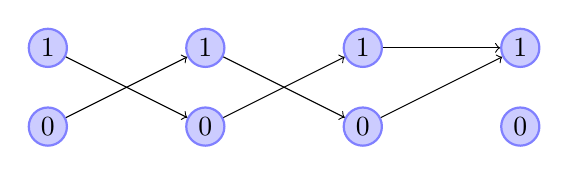
\begin{tikzpicture}
  [state/.style={circle, draw=blue!50, fill=blue!20, thick, inner sep=2pt}]
  \foreach \x in {0, 2, 4, 6}{
    \node (n1\x) at (\x, 1) [state] {1};
    \node (n0\x) at (\x, 0) [state] {0};
  }
  \draw [->] (n10) to (n02);
  \draw [->] (n00) to (n12);
  \draw [->] (n12) to (n04);
  \draw [->] (n02) to (n14);
  \draw [->] (n14) to (n16);
  \draw [->] (n04) to (n16);
\end{tikzpicture}
\end{center}

\paragraph{Coupling From The Past with no Memory}
It is quite nature to implement the CFTP sampler without \textbf{reuse}, but unfortunately, this variation of CFTP is wrong.
This sampler covers all the cases, but it does not follow the right distribution.
The probobility of this sampler returns sample $s$ equals:
\begin{align*}
&\sum_{T=1}^\infty \Pr[\mbox{$f$ has constant $s$ $|$ $\substack{\mbox{$f$ is a constant function in $T$}\\ \mbox{$\land$ $f$ is not a constant function in $\{1, \cdots, T-1\}$}}$}] \\
                  &= \sum_{T=1}^\infty \Pr[\mbox{$f$ has constant $s$ $|$ sampler halts in $T$ steps}] \Pr[\mbox{sampler halts in $T$ steps}] \\
  &= \sum_{T=1}^\infty \frac{\Pr[\mbox{constant function in $T$ steps with constant $s$}]}{\Pr[\mbox{function in $T$ steps}]} \prod_{t=1}^{T-1}\frac{\Pr[\mbox{$t$ steps not constant function}]}{\Pr[\mbox{function in $t$ steps}]} \\
\end{align*}
Actually, its hard to find any relationship between this distribution and the correct distribution.
When $s = 1$, then using the example above, we have
\begin{align*}
  \Pr[s = 1] &\geq \textcolor{red}{\Pr[\mbox{1 step}]}\textcolor{blue}{\Pr[\mbox{$f$ has constant $1$} | \mbox{1 step}]} + \textcolor{cyan}{\Pr[\mbox{2 steps}]}\textcolor{blue!50}{\Pr[\mbox{$f$ has constant $1$} | \mbox{2 steps}]} \\
             &= \textcolor{red}{\frac{1}{2}}\cdot \textcolor{blue}{1} + \textcolor{cyan}{\frac{1}{2}\cdot\frac{3}{4}}\cdot\textcolor{blue!50}{\frac{2}{3}} \\
  &= \frac{3}{4} > \frac{2}{3}
\end{align*}
So, its easy to see that this sampler does not catch the right distribution.

\begin{center}
\begin{tikzpicture}
  [state/.style={circle, draw=blue!50, fill=blue!20, thick, inner sep=2pt}]
  \foreach \x in {0, 2}{
    \node (n1\x) at (\x, 1) [state] {1};
    \node (n0\x) at (\x, 0) [state] {0};
  }
  \draw [->] (n10) to (n02);
  \draw [->] (n00) to (n12);
\end{tikzpicture} \hspace{0.5cm}
\begin{tikzpicture}
  [state/.style={circle, draw=blue!50, fill=blue!20, thick, inner sep=2pt}]
  \foreach \x in {0, 2}{
    \node (n1\x) at (\x, 1) [state] {1};
    \node (n0\x) at (\x, 0) [state] {0};
  }
  \draw [->] (n10) to (n12);
  \draw [->] (n00) to (n12);
\end{tikzpicture}
\end{center}

\begin{center}
\begin{tikzpicture}
  [state/.style={circle, draw=blue!50, fill=blue!20, thick, inner sep=2pt}]
  \foreach \x in {0, 2, 4}{
    \node (n1\x) at (\x, 1) [state] {1};
    \node (n0\x) at (\x, 0) [state] {0};
  }
  \draw [->] (n10) to (n02);
  \draw [->] (n00) to (n12);
  \draw [->] (n12) to (n04);
  \draw [->] (n02) to (n14);
\end{tikzpicture} \hspace{0.5cm}
\begin{tikzpicture}
  [state/.style={circle, draw=blue!50, fill=blue!20, thick, inner sep=2pt}]
  \foreach \x in {0, 2, 4}{
    \node (n1\x) at (\x, 1) [state] {1};
    \node (n0\x) at (\x, 0) [state] {0};
  }
  \draw [->] (n10) to (n02);
  \draw [->] (n00) to (n12);
  \draw [->] (n12) to (n14);
  \draw [->] (n02) to (n14);
\end{tikzpicture} \vspace{0.5cm} \\
\begin{tikzpicture}
  [state/.style={circle, draw=blue!50, fill=blue!20, thick, inner sep=2pt}]
  \foreach \x in {0, 2, 4}{
    \node (n1\x) at (\x, 1) [state] {1};
    \node (n0\x) at (\x, 0) [state] {0};
  }
  \draw [->] (n10) to (n12);
  \draw [->] (n00) to (n12);
  \draw [->] (n12) to (n04);
  \draw [->] (n02) to (n14);
\end{tikzpicture} \hspace{0.5cm}
\begin{tikzpicture}
  [state/.style={circle, draw=blue!50, fill=blue!20, thick, inner sep=2pt}]
  \foreach \x in {0, 2, 4}{
    \node (n1\x) at (\x, 1) [state] {1};
    \node (n0\x) at (\x, 0) [state] {0};
  }
  \draw [->] (n10) to (n12);
  \draw [->] (n00) to (n12);
  \draw [->] (n12) to (n14);
  \draw [->] (n02) to (n14);
\end{tikzpicture} 
\end{center}
%%% Local Variables:
%%% mode: latex
%%% TeX-master: "../../notebook"
%%% End:


% what is Gamma function and some useful tricks
\section{Coupling From the Past}
\paragraph{}
Coupling from the past (CFTP) is a method with which we could perform a perfect sampling according to some distribution.
I can not find any convincing proof of this result, so I decide to prove it myself.

First, lets view Markov Chain in a new but nature way.
Suppose we have a Markov Chain $\mathcal{M}$ defined on some state set $S = \{s_1, s_2, \cdots, s_n\}$.
Note that when we execute $\mathcal{M}$, then in each turn, this chain will fix some parameters according to some distribution and move from some states to other states.
So, if we fix this random parameters, then $\mathcal{M}$ becomes a determined process, and we could view it as a function $f: S\to S$. For convenience, lets denote the determined process from time $i$ to time $i+1$ by $f_i$.
The pseudocode of CFTP is shown below.
\begin{algorithm}
  Coupling From The Past () \Begin{
    $T \gets 1$ \\
    \Repeat{$f$ becomes a constant function}{
      $f \gets f_{-T} \circ f_{-(T-1)} \circ \cdots \circ f_{-1}$ \\
      $T \gets T + 1$
    }
    \Return{$f(s_1)$}
  }
\end{algorithm}
\marginnote[-3cm]{The $\circ$ here means compose operator where $f \circ g  (x) = g(f(x))$, i.e. give $f$'s output as $g$'s input.}
\marginnote[-1.8cm]{Here, $f_{-i}$ is fixed (by random) at the first time we encountered it, and will be \textbf{reused} later.}

The idea of this sampler is quite simple.
Suppose we have a Markov Chain $\mathcal{M}$ which starts at $-\infty$ and stops at $0$, then its pretty sure that it will have the distribution $\pi$ at time $0$ (no matter which state it starts from).
Then, if we randomly determine some last finite steps of the chain (say $T$ steps), we may have the chance to recover the sample of this MC by this steps.

And, its quite easy to see that when the last $T$ steps forms a constant function we could easily recover the sample from this MC. So we have the following theorem:
\begin{theorem}
  If we have a Markov Chain $\mathcal{M}$ such that
  \[\lim_{t\to\infty} \Pr [f_0 \circ f_1 \circ \cdots \circ f_t \mbox{ is a constant function}] = 1\]
  where $f_0, f_1, \cdots, f_t$ are fixed randomly according to the transition matrix $P$ of $\mathcal{M}$,
  then the CFTP of $\mathcal{M}$ halt in finite time with probability $1$ and returns a sample according to $\pi$.
\end{theorem}
\begin{proof}
  Note that, if our algorithm could \textbf{cover} all the cases of the last finite steps of the Markov Chain, and could \textbf{recover} the sample from all these cases, then its easy to see, this algorithm should be right.

  So, here, its quite nature to ask, what means all the cases?
  Here, a case is a suffix of the chain from $-\infty$ to $0$.
  Note that, CFTP randomly choose a $f_{-t}$ at time $-t$, so if we omit the stop condition, its should cover all the cases.
  Suppose the CFTP stops at some time $T$, which means its forms a constant function $f$ and no matter how we extend this suffix, this constant will not change, so we could pack all the suffix that end with this suffix into this suffix, since they have the same sample (while do not change the distribution of sample).
  Hence, CFTP forms a cover of all the cases.

  Since $\lim_{t\to\infty}\Pr[f_0\circ f_1\circ \cdots\circ f_t] = 1$, the Markov Chain will be a constant function with probability 1 after infinite steps. Which notes us that CFTP should halt in finite time with probability $1$.
  
  Finally, since CFTP simulates a Markov Chain which have been executed for infinite steps, so the distribution of the sample should be exactly $\pi$.
\end{proof}

\subsection{Two confusing bad variations of CFTP}
\paragraph{Coupling to the future}
Its nature for us to ask, ``why not just coupling to the future?'', since this two samplers look nearly the same.
\begin{algorithm}
  Copuling To The Future () \Begin{
    $T\gets 1$ \\
    \Repeat{$f$ becomes a constant function}{
      $f \gets f_0\circ f_1\circ \cdots \circ f_T$ \\
      $T\gets T+1$
    }
    \Return{$f(s_1)$}
  }
\end{algorithm}

The problem here is that is sampler does not cover all the cases.
First, if we omit the stop condition, then it is easy to see that this sampler covers all the cases. Similarly, this sampler want to pack some of the cases so that we could stop in finite steps. Note that, if $f$ becomes a constant function in time $T$, then $f'$ will also be a constant function in time $T+1$ and so on. But $f$ and $f'$ has different constant, so we could not pack them together (we should not use the sample of $f$ to represent the sample of $f'$).
So, there is a bias in the result distribution.

Here is a quite simple example to explain this:
Suppose we have a Markov chain with state space $[2] = \{1, 2\}$ and transition matrix
\[P = \left[
    \begin{array}{cc}
      0.5 & 0.5 \\
      1   & 0
    \end{array}
  \right]\]
Obviously, $\pi = (\pi_1, \pi_2) = (\frac{2}{3}, \frac{1}{3})$.
In this example, the \emph{coupling to the future} sampler always returns $1$ as its result.

\begin{center}
\begin{tikzpicture}
  [state/.style={circle, draw=blue!50, fill=blue!20, thick, inner sep=2pt}]
  \foreach \x in {0, 2, 4, 6}{
    \node (n1\x) at (\x, 1) [state] {1};
    \node (n0\x) at (\x, 0) [state] {0};
  }
  \draw [->] (n10) to (n02);
  \draw [->] (n00) to (n12);
  \draw [->] (n12) to (n04);
  \draw [->] (n02) to (n14);
  \draw [->] (n14) to (n16);
  \draw [->] (n04) to (n16);
\end{tikzpicture}
\end{center}

\paragraph{Coupling From The Past with no Memory}
It is quite nature to implement the CFTP sampler without \textbf{reuse}, but unfortunately, this variation of CFTP is wrong.
This sampler covers all the cases, but it does not follow the right distribution.
The probobility of this sampler returns sample $s$ equals:
\begin{align*}
&\sum_{T=1}^\infty \Pr[\mbox{$f$ has constant $s$ $|$ $\substack{\mbox{$f$ is a constant function in $T$}\\ \mbox{$\land$ $f$ is not a constant function in $\{1, \cdots, T-1\}$}}$}] \\
                  &= \sum_{T=1}^\infty \Pr[\mbox{$f$ has constant $s$ $|$ sampler halts in $T$ steps}] \Pr[\mbox{sampler halts in $T$ steps}] \\
  &= \sum_{T=1}^\infty \frac{\Pr[\mbox{constant function in $T$ steps with constant $s$}]}{\Pr[\mbox{function in $T$ steps}]} \prod_{t=1}^{T-1}\frac{\Pr[\mbox{$t$ steps not constant function}]}{\Pr[\mbox{function in $t$ steps}]} \\
\end{align*}
Actually, its hard to find any relationship between this distribution and the correct distribution.
When $s = 1$, then using the example above, we have
\begin{align*}
  \Pr[s = 1] &\geq \textcolor{red}{\Pr[\mbox{1 step}]}\textcolor{blue}{\Pr[\mbox{$f$ has constant $1$} | \mbox{1 step}]} + \textcolor{cyan}{\Pr[\mbox{2 steps}]}\textcolor{blue!50}{\Pr[\mbox{$f$ has constant $1$} | \mbox{2 steps}]} \\
             &= \textcolor{red}{\frac{1}{2}}\cdot \textcolor{blue}{1} + \textcolor{cyan}{\frac{1}{2}\cdot\frac{3}{4}}\cdot\textcolor{blue!50}{\frac{2}{3}} \\
  &= \frac{3}{4} > \frac{2}{3}
\end{align*}
So, its easy to see that this sampler does not catch the right distribution.

\begin{center}
\begin{tikzpicture}
  [state/.style={circle, draw=blue!50, fill=blue!20, thick, inner sep=2pt}]
  \foreach \x in {0, 2}{
    \node (n1\x) at (\x, 1) [state] {1};
    \node (n0\x) at (\x, 0) [state] {0};
  }
  \draw [->] (n10) to (n02);
  \draw [->] (n00) to (n12);
\end{tikzpicture} \hspace{0.5cm}
\begin{tikzpicture}
  [state/.style={circle, draw=blue!50, fill=blue!20, thick, inner sep=2pt}]
  \foreach \x in {0, 2}{
    \node (n1\x) at (\x, 1) [state] {1};
    \node (n0\x) at (\x, 0) [state] {0};
  }
  \draw [->] (n10) to (n12);
  \draw [->] (n00) to (n12);
\end{tikzpicture}
\end{center}

\begin{center}
\begin{tikzpicture}
  [state/.style={circle, draw=blue!50, fill=blue!20, thick, inner sep=2pt}]
  \foreach \x in {0, 2, 4}{
    \node (n1\x) at (\x, 1) [state] {1};
    \node (n0\x) at (\x, 0) [state] {0};
  }
  \draw [->] (n10) to (n02);
  \draw [->] (n00) to (n12);
  \draw [->] (n12) to (n04);
  \draw [->] (n02) to (n14);
\end{tikzpicture} \hspace{0.5cm}
\begin{tikzpicture}
  [state/.style={circle, draw=blue!50, fill=blue!20, thick, inner sep=2pt}]
  \foreach \x in {0, 2, 4}{
    \node (n1\x) at (\x, 1) [state] {1};
    \node (n0\x) at (\x, 0) [state] {0};
  }
  \draw [->] (n10) to (n02);
  \draw [->] (n00) to (n12);
  \draw [->] (n12) to (n14);
  \draw [->] (n02) to (n14);
\end{tikzpicture} \vspace{0.5cm} \\
\begin{tikzpicture}
  [state/.style={circle, draw=blue!50, fill=blue!20, thick, inner sep=2pt}]
  \foreach \x in {0, 2, 4}{
    \node (n1\x) at (\x, 1) [state] {1};
    \node (n0\x) at (\x, 0) [state] {0};
  }
  \draw [->] (n10) to (n12);
  \draw [->] (n00) to (n12);
  \draw [->] (n12) to (n04);
  \draw [->] (n02) to (n14);
\end{tikzpicture} \hspace{0.5cm}
\begin{tikzpicture}
  [state/.style={circle, draw=blue!50, fill=blue!20, thick, inner sep=2pt}]
  \foreach \x in {0, 2, 4}{
    \node (n1\x) at (\x, 1) [state] {1};
    \node (n0\x) at (\x, 0) [state] {0};
  }
  \draw [->] (n10) to (n12);
  \draw [->] (n00) to (n12);
  \draw [->] (n12) to (n14);
  \draw [->] (n02) to (n14);
\end{tikzpicture} 
\end{center}
%%% Local Variables:
%%% mode: latex
%%% TeX-master: "../../notebook"
%%% End:


% some tricks for the total variation distance
\section{Coupling From the Past}
\paragraph{}
Coupling from the past (CFTP) is a method with which we could perform a perfect sampling according to some distribution.
I can not find any convincing proof of this result, so I decide to prove it myself.

First, lets view Markov Chain in a new but nature way.
Suppose we have a Markov Chain $\mathcal{M}$ defined on some state set $S = \{s_1, s_2, \cdots, s_n\}$.
Note that when we execute $\mathcal{M}$, then in each turn, this chain will fix some parameters according to some distribution and move from some states to other states.
So, if we fix this random parameters, then $\mathcal{M}$ becomes a determined process, and we could view it as a function $f: S\to S$. For convenience, lets denote the determined process from time $i$ to time $i+1$ by $f_i$.
The pseudocode of CFTP is shown below.
\begin{algorithm}
  Coupling From The Past () \Begin{
    $T \gets 1$ \\
    \Repeat{$f$ becomes a constant function}{
      $f \gets f_{-T} \circ f_{-(T-1)} \circ \cdots \circ f_{-1}$ \\
      $T \gets T + 1$
    }
    \Return{$f(s_1)$}
  }
\end{algorithm}
\marginnote[-3cm]{The $\circ$ here means compose operator where $f \circ g  (x) = g(f(x))$, i.e. give $f$'s output as $g$'s input.}
\marginnote[-1.8cm]{Here, $f_{-i}$ is fixed (by random) at the first time we encountered it, and will be \textbf{reused} later.}

The idea of this sampler is quite simple.
Suppose we have a Markov Chain $\mathcal{M}$ which starts at $-\infty$ and stops at $0$, then its pretty sure that it will have the distribution $\pi$ at time $0$ (no matter which state it starts from).
Then, if we randomly determine some last finite steps of the chain (say $T$ steps), we may have the chance to recover the sample of this MC by this steps.

And, its quite easy to see that when the last $T$ steps forms a constant function we could easily recover the sample from this MC. So we have the following theorem:
\begin{theorem}
  If we have a Markov Chain $\mathcal{M}$ such that
  \[\lim_{t\to\infty} \Pr [f_0 \circ f_1 \circ \cdots \circ f_t \mbox{ is a constant function}] = 1\]
  where $f_0, f_1, \cdots, f_t$ are fixed randomly according to the transition matrix $P$ of $\mathcal{M}$,
  then the CFTP of $\mathcal{M}$ halt in finite time with probability $1$ and returns a sample according to $\pi$.
\end{theorem}
\begin{proof}
  Note that, if our algorithm could \textbf{cover} all the cases of the last finite steps of the Markov Chain, and could \textbf{recover} the sample from all these cases, then its easy to see, this algorithm should be right.

  So, here, its quite nature to ask, what means all the cases?
  Here, a case is a suffix of the chain from $-\infty$ to $0$.
  Note that, CFTP randomly choose a $f_{-t}$ at time $-t$, so if we omit the stop condition, its should cover all the cases.
  Suppose the CFTP stops at some time $T$, which means its forms a constant function $f$ and no matter how we extend this suffix, this constant will not change, so we could pack all the suffix that end with this suffix into this suffix, since they have the same sample (while do not change the distribution of sample).
  Hence, CFTP forms a cover of all the cases.

  Since $\lim_{t\to\infty}\Pr[f_0\circ f_1\circ \cdots\circ f_t] = 1$, the Markov Chain will be a constant function with probability 1 after infinite steps. Which notes us that CFTP should halt in finite time with probability $1$.
  
  Finally, since CFTP simulates a Markov Chain which have been executed for infinite steps, so the distribution of the sample should be exactly $\pi$.
\end{proof}

\subsection{Two confusing bad variations of CFTP}
\paragraph{Coupling to the future}
Its nature for us to ask, ``why not just coupling to the future?'', since this two samplers look nearly the same.
\begin{algorithm}
  Copuling To The Future () \Begin{
    $T\gets 1$ \\
    \Repeat{$f$ becomes a constant function}{
      $f \gets f_0\circ f_1\circ \cdots \circ f_T$ \\
      $T\gets T+1$
    }
    \Return{$f(s_1)$}
  }
\end{algorithm}

The problem here is that is sampler does not cover all the cases.
First, if we omit the stop condition, then it is easy to see that this sampler covers all the cases. Similarly, this sampler want to pack some of the cases so that we could stop in finite steps. Note that, if $f$ becomes a constant function in time $T$, then $f'$ will also be a constant function in time $T+1$ and so on. But $f$ and $f'$ has different constant, so we could not pack them together (we should not use the sample of $f$ to represent the sample of $f'$).
So, there is a bias in the result distribution.

Here is a quite simple example to explain this:
Suppose we have a Markov chain with state space $[2] = \{1, 2\}$ and transition matrix
\[P = \left[
    \begin{array}{cc}
      0.5 & 0.5 \\
      1   & 0
    \end{array}
  \right]\]
Obviously, $\pi = (\pi_1, \pi_2) = (\frac{2}{3}, \frac{1}{3})$.
In this example, the \emph{coupling to the future} sampler always returns $1$ as its result.

\begin{center}
\begin{tikzpicture}
  [state/.style={circle, draw=blue!50, fill=blue!20, thick, inner sep=2pt}]
  \foreach \x in {0, 2, 4, 6}{
    \node (n1\x) at (\x, 1) [state] {1};
    \node (n0\x) at (\x, 0) [state] {0};
  }
  \draw [->] (n10) to (n02);
  \draw [->] (n00) to (n12);
  \draw [->] (n12) to (n04);
  \draw [->] (n02) to (n14);
  \draw [->] (n14) to (n16);
  \draw [->] (n04) to (n16);
\end{tikzpicture}
\end{center}

\paragraph{Coupling From The Past with no Memory}
It is quite nature to implement the CFTP sampler without \textbf{reuse}, but unfortunately, this variation of CFTP is wrong.
This sampler covers all the cases, but it does not follow the right distribution.
The probobility of this sampler returns sample $s$ equals:
\begin{align*}
&\sum_{T=1}^\infty \Pr[\mbox{$f$ has constant $s$ $|$ $\substack{\mbox{$f$ is a constant function in $T$}\\ \mbox{$\land$ $f$ is not a constant function in $\{1, \cdots, T-1\}$}}$}] \\
                  &= \sum_{T=1}^\infty \Pr[\mbox{$f$ has constant $s$ $|$ sampler halts in $T$ steps}] \Pr[\mbox{sampler halts in $T$ steps}] \\
  &= \sum_{T=1}^\infty \frac{\Pr[\mbox{constant function in $T$ steps with constant $s$}]}{\Pr[\mbox{function in $T$ steps}]} \prod_{t=1}^{T-1}\frac{\Pr[\mbox{$t$ steps not constant function}]}{\Pr[\mbox{function in $t$ steps}]} \\
\end{align*}
Actually, its hard to find any relationship between this distribution and the correct distribution.
When $s = 1$, then using the example above, we have
\begin{align*}
  \Pr[s = 1] &\geq \textcolor{red}{\Pr[\mbox{1 step}]}\textcolor{blue}{\Pr[\mbox{$f$ has constant $1$} | \mbox{1 step}]} + \textcolor{cyan}{\Pr[\mbox{2 steps}]}\textcolor{blue!50}{\Pr[\mbox{$f$ has constant $1$} | \mbox{2 steps}]} \\
             &= \textcolor{red}{\frac{1}{2}}\cdot \textcolor{blue}{1} + \textcolor{cyan}{\frac{1}{2}\cdot\frac{3}{4}}\cdot\textcolor{blue!50}{\frac{2}{3}} \\
  &= \frac{3}{4} > \frac{2}{3}
\end{align*}
So, its easy to see that this sampler does not catch the right distribution.

\begin{center}
\begin{tikzpicture}
  [state/.style={circle, draw=blue!50, fill=blue!20, thick, inner sep=2pt}]
  \foreach \x in {0, 2}{
    \node (n1\x) at (\x, 1) [state] {1};
    \node (n0\x) at (\x, 0) [state] {0};
  }
  \draw [->] (n10) to (n02);
  \draw [->] (n00) to (n12);
\end{tikzpicture} \hspace{0.5cm}
\begin{tikzpicture}
  [state/.style={circle, draw=blue!50, fill=blue!20, thick, inner sep=2pt}]
  \foreach \x in {0, 2}{
    \node (n1\x) at (\x, 1) [state] {1};
    \node (n0\x) at (\x, 0) [state] {0};
  }
  \draw [->] (n10) to (n12);
  \draw [->] (n00) to (n12);
\end{tikzpicture}
\end{center}

\begin{center}
\begin{tikzpicture}
  [state/.style={circle, draw=blue!50, fill=blue!20, thick, inner sep=2pt}]
  \foreach \x in {0, 2, 4}{
    \node (n1\x) at (\x, 1) [state] {1};
    \node (n0\x) at (\x, 0) [state] {0};
  }
  \draw [->] (n10) to (n02);
  \draw [->] (n00) to (n12);
  \draw [->] (n12) to (n04);
  \draw [->] (n02) to (n14);
\end{tikzpicture} \hspace{0.5cm}
\begin{tikzpicture}
  [state/.style={circle, draw=blue!50, fill=blue!20, thick, inner sep=2pt}]
  \foreach \x in {0, 2, 4}{
    \node (n1\x) at (\x, 1) [state] {1};
    \node (n0\x) at (\x, 0) [state] {0};
  }
  \draw [->] (n10) to (n02);
  \draw [->] (n00) to (n12);
  \draw [->] (n12) to (n14);
  \draw [->] (n02) to (n14);
\end{tikzpicture} \vspace{0.5cm} \\
\begin{tikzpicture}
  [state/.style={circle, draw=blue!50, fill=blue!20, thick, inner sep=2pt}]
  \foreach \x in {0, 2, 4}{
    \node (n1\x) at (\x, 1) [state] {1};
    \node (n0\x) at (\x, 0) [state] {0};
  }
  \draw [->] (n10) to (n12);
  \draw [->] (n00) to (n12);
  \draw [->] (n12) to (n04);
  \draw [->] (n02) to (n14);
\end{tikzpicture} \hspace{0.5cm}
\begin{tikzpicture}
  [state/.style={circle, draw=blue!50, fill=blue!20, thick, inner sep=2pt}]
  \foreach \x in {0, 2, 4}{
    \node (n1\x) at (\x, 1) [state] {1};
    \node (n0\x) at (\x, 0) [state] {0};
  }
  \draw [->] (n10) to (n12);
  \draw [->] (n00) to (n12);
  \draw [->] (n12) to (n14);
  \draw [->] (n02) to (n14);
\end{tikzpicture} 
\end{center}
%%% Local Variables:
%%% mode: latex
%%% TeX-master: "../../notebook"
%%% End:


% Chebyshev inequality
\section{Coupling From the Past}
\paragraph{}
Coupling from the past (CFTP) is a method with which we could perform a perfect sampling according to some distribution.
I can not find any convincing proof of this result, so I decide to prove it myself.

First, lets view Markov Chain in a new but nature way.
Suppose we have a Markov Chain $\mathcal{M}$ defined on some state set $S = \{s_1, s_2, \cdots, s_n\}$.
Note that when we execute $\mathcal{M}$, then in each turn, this chain will fix some parameters according to some distribution and move from some states to other states.
So, if we fix this random parameters, then $\mathcal{M}$ becomes a determined process, and we could view it as a function $f: S\to S$. For convenience, lets denote the determined process from time $i$ to time $i+1$ by $f_i$.
The pseudocode of CFTP is shown below.
\begin{algorithm}
  Coupling From The Past () \Begin{
    $T \gets 1$ \\
    \Repeat{$f$ becomes a constant function}{
      $f \gets f_{-T} \circ f_{-(T-1)} \circ \cdots \circ f_{-1}$ \\
      $T \gets T + 1$
    }
    \Return{$f(s_1)$}
  }
\end{algorithm}
\marginnote[-3cm]{The $\circ$ here means compose operator where $f \circ g  (x) = g(f(x))$, i.e. give $f$'s output as $g$'s input.}
\marginnote[-1.8cm]{Here, $f_{-i}$ is fixed (by random) at the first time we encountered it, and will be \textbf{reused} later.}

The idea of this sampler is quite simple.
Suppose we have a Markov Chain $\mathcal{M}$ which starts at $-\infty$ and stops at $0$, then its pretty sure that it will have the distribution $\pi$ at time $0$ (no matter which state it starts from).
Then, if we randomly determine some last finite steps of the chain (say $T$ steps), we may have the chance to recover the sample of this MC by this steps.

And, its quite easy to see that when the last $T$ steps forms a constant function we could easily recover the sample from this MC. So we have the following theorem:
\begin{theorem}
  If we have a Markov Chain $\mathcal{M}$ such that
  \[\lim_{t\to\infty} \Pr [f_0 \circ f_1 \circ \cdots \circ f_t \mbox{ is a constant function}] = 1\]
  where $f_0, f_1, \cdots, f_t$ are fixed randomly according to the transition matrix $P$ of $\mathcal{M}$,
  then the CFTP of $\mathcal{M}$ halt in finite time with probability $1$ and returns a sample according to $\pi$.
\end{theorem}
\begin{proof}
  Note that, if our algorithm could \textbf{cover} all the cases of the last finite steps of the Markov Chain, and could \textbf{recover} the sample from all these cases, then its easy to see, this algorithm should be right.

  So, here, its quite nature to ask, what means all the cases?
  Here, a case is a suffix of the chain from $-\infty$ to $0$.
  Note that, CFTP randomly choose a $f_{-t}$ at time $-t$, so if we omit the stop condition, its should cover all the cases.
  Suppose the CFTP stops at some time $T$, which means its forms a constant function $f$ and no matter how we extend this suffix, this constant will not change, so we could pack all the suffix that end with this suffix into this suffix, since they have the same sample (while do not change the distribution of sample).
  Hence, CFTP forms a cover of all the cases.

  Since $\lim_{t\to\infty}\Pr[f_0\circ f_1\circ \cdots\circ f_t] = 1$, the Markov Chain will be a constant function with probability 1 after infinite steps. Which notes us that CFTP should halt in finite time with probability $1$.
  
  Finally, since CFTP simulates a Markov Chain which have been executed for infinite steps, so the distribution of the sample should be exactly $\pi$.
\end{proof}

\subsection{Two confusing bad variations of CFTP}
\paragraph{Coupling to the future}
Its nature for us to ask, ``why not just coupling to the future?'', since this two samplers look nearly the same.
\begin{algorithm}
  Copuling To The Future () \Begin{
    $T\gets 1$ \\
    \Repeat{$f$ becomes a constant function}{
      $f \gets f_0\circ f_1\circ \cdots \circ f_T$ \\
      $T\gets T+1$
    }
    \Return{$f(s_1)$}
  }
\end{algorithm}

The problem here is that is sampler does not cover all the cases.
First, if we omit the stop condition, then it is easy to see that this sampler covers all the cases. Similarly, this sampler want to pack some of the cases so that we could stop in finite steps. Note that, if $f$ becomes a constant function in time $T$, then $f'$ will also be a constant function in time $T+1$ and so on. But $f$ and $f'$ has different constant, so we could not pack them together (we should not use the sample of $f$ to represent the sample of $f'$).
So, there is a bias in the result distribution.

Here is a quite simple example to explain this:
Suppose we have a Markov chain with state space $[2] = \{1, 2\}$ and transition matrix
\[P = \left[
    \begin{array}{cc}
      0.5 & 0.5 \\
      1   & 0
    \end{array}
  \right]\]
Obviously, $\pi = (\pi_1, \pi_2) = (\frac{2}{3}, \frac{1}{3})$.
In this example, the \emph{coupling to the future} sampler always returns $1$ as its result.

\begin{center}
\begin{tikzpicture}
  [state/.style={circle, draw=blue!50, fill=blue!20, thick, inner sep=2pt}]
  \foreach \x in {0, 2, 4, 6}{
    \node (n1\x) at (\x, 1) [state] {1};
    \node (n0\x) at (\x, 0) [state] {0};
  }
  \draw [->] (n10) to (n02);
  \draw [->] (n00) to (n12);
  \draw [->] (n12) to (n04);
  \draw [->] (n02) to (n14);
  \draw [->] (n14) to (n16);
  \draw [->] (n04) to (n16);
\end{tikzpicture}
\end{center}

\paragraph{Coupling From The Past with no Memory}
It is quite nature to implement the CFTP sampler without \textbf{reuse}, but unfortunately, this variation of CFTP is wrong.
This sampler covers all the cases, but it does not follow the right distribution.
The probobility of this sampler returns sample $s$ equals:
\begin{align*}
&\sum_{T=1}^\infty \Pr[\mbox{$f$ has constant $s$ $|$ $\substack{\mbox{$f$ is a constant function in $T$}\\ \mbox{$\land$ $f$ is not a constant function in $\{1, \cdots, T-1\}$}}$}] \\
                  &= \sum_{T=1}^\infty \Pr[\mbox{$f$ has constant $s$ $|$ sampler halts in $T$ steps}] \Pr[\mbox{sampler halts in $T$ steps}] \\
  &= \sum_{T=1}^\infty \frac{\Pr[\mbox{constant function in $T$ steps with constant $s$}]}{\Pr[\mbox{function in $T$ steps}]} \prod_{t=1}^{T-1}\frac{\Pr[\mbox{$t$ steps not constant function}]}{\Pr[\mbox{function in $t$ steps}]} \\
\end{align*}
Actually, its hard to find any relationship between this distribution and the correct distribution.
When $s = 1$, then using the example above, we have
\begin{align*}
  \Pr[s = 1] &\geq \textcolor{red}{\Pr[\mbox{1 step}]}\textcolor{blue}{\Pr[\mbox{$f$ has constant $1$} | \mbox{1 step}]} + \textcolor{cyan}{\Pr[\mbox{2 steps}]}\textcolor{blue!50}{\Pr[\mbox{$f$ has constant $1$} | \mbox{2 steps}]} \\
             &= \textcolor{red}{\frac{1}{2}}\cdot \textcolor{blue}{1} + \textcolor{cyan}{\frac{1}{2}\cdot\frac{3}{4}}\cdot\textcolor{blue!50}{\frac{2}{3}} \\
  &= \frac{3}{4} > \frac{2}{3}
\end{align*}
So, its easy to see that this sampler does not catch the right distribution.

\begin{center}
\begin{tikzpicture}
  [state/.style={circle, draw=blue!50, fill=blue!20, thick, inner sep=2pt}]
  \foreach \x in {0, 2}{
    \node (n1\x) at (\x, 1) [state] {1};
    \node (n0\x) at (\x, 0) [state] {0};
  }
  \draw [->] (n10) to (n02);
  \draw [->] (n00) to (n12);
\end{tikzpicture} \hspace{0.5cm}
\begin{tikzpicture}
  [state/.style={circle, draw=blue!50, fill=blue!20, thick, inner sep=2pt}]
  \foreach \x in {0, 2}{
    \node (n1\x) at (\x, 1) [state] {1};
    \node (n0\x) at (\x, 0) [state] {0};
  }
  \draw [->] (n10) to (n12);
  \draw [->] (n00) to (n12);
\end{tikzpicture}
\end{center}

\begin{center}
\begin{tikzpicture}
  [state/.style={circle, draw=blue!50, fill=blue!20, thick, inner sep=2pt}]
  \foreach \x in {0, 2, 4}{
    \node (n1\x) at (\x, 1) [state] {1};
    \node (n0\x) at (\x, 0) [state] {0};
  }
  \draw [->] (n10) to (n02);
  \draw [->] (n00) to (n12);
  \draw [->] (n12) to (n04);
  \draw [->] (n02) to (n14);
\end{tikzpicture} \hspace{0.5cm}
\begin{tikzpicture}
  [state/.style={circle, draw=blue!50, fill=blue!20, thick, inner sep=2pt}]
  \foreach \x in {0, 2, 4}{
    \node (n1\x) at (\x, 1) [state] {1};
    \node (n0\x) at (\x, 0) [state] {0};
  }
  \draw [->] (n10) to (n02);
  \draw [->] (n00) to (n12);
  \draw [->] (n12) to (n14);
  \draw [->] (n02) to (n14);
\end{tikzpicture} \vspace{0.5cm} \\
\begin{tikzpicture}
  [state/.style={circle, draw=blue!50, fill=blue!20, thick, inner sep=2pt}]
  \foreach \x in {0, 2, 4}{
    \node (n1\x) at (\x, 1) [state] {1};
    \node (n0\x) at (\x, 0) [state] {0};
  }
  \draw [->] (n10) to (n12);
  \draw [->] (n00) to (n12);
  \draw [->] (n12) to (n04);
  \draw [->] (n02) to (n14);
\end{tikzpicture} \hspace{0.5cm}
\begin{tikzpicture}
  [state/.style={circle, draw=blue!50, fill=blue!20, thick, inner sep=2pt}]
  \foreach \x in {0, 2, 4}{
    \node (n1\x) at (\x, 1) [state] {1};
    \node (n0\x) at (\x, 0) [state] {0};
  }
  \draw [->] (n10) to (n12);
  \draw [->] (n00) to (n12);
  \draw [->] (n12) to (n14);
  \draw [->] (n02) to (n14);
\end{tikzpicture} 
\end{center}
%%% Local Variables:
%%% mode: latex
%%% TeX-master: "../../notebook"
%%% End:


\chapter{Topics Related to Geometry}
\clearpage

% Radon's Theorem
\section{Coupling From the Past}
\paragraph{}
Coupling from the past (CFTP) is a method with which we could perform a perfect sampling according to some distribution.
I can not find any convincing proof of this result, so I decide to prove it myself.

First, lets view Markov Chain in a new but nature way.
Suppose we have a Markov Chain $\mathcal{M}$ defined on some state set $S = \{s_1, s_2, \cdots, s_n\}$.
Note that when we execute $\mathcal{M}$, then in each turn, this chain will fix some parameters according to some distribution and move from some states to other states.
So, if we fix this random parameters, then $\mathcal{M}$ becomes a determined process, and we could view it as a function $f: S\to S$. For convenience, lets denote the determined process from time $i$ to time $i+1$ by $f_i$.
The pseudocode of CFTP is shown below.
\begin{algorithm}
  Coupling From The Past () \Begin{
    $T \gets 1$ \\
    \Repeat{$f$ becomes a constant function}{
      $f \gets f_{-T} \circ f_{-(T-1)} \circ \cdots \circ f_{-1}$ \\
      $T \gets T + 1$
    }
    \Return{$f(s_1)$}
  }
\end{algorithm}
\marginnote[-3cm]{The $\circ$ here means compose operator where $f \circ g  (x) = g(f(x))$, i.e. give $f$'s output as $g$'s input.}
\marginnote[-1.8cm]{Here, $f_{-i}$ is fixed (by random) at the first time we encountered it, and will be \textbf{reused} later.}

The idea of this sampler is quite simple.
Suppose we have a Markov Chain $\mathcal{M}$ which starts at $-\infty$ and stops at $0$, then its pretty sure that it will have the distribution $\pi$ at time $0$ (no matter which state it starts from).
Then, if we randomly determine some last finite steps of the chain (say $T$ steps), we may have the chance to recover the sample of this MC by this steps.

And, its quite easy to see that when the last $T$ steps forms a constant function we could easily recover the sample from this MC. So we have the following theorem:
\begin{theorem}
  If we have a Markov Chain $\mathcal{M}$ such that
  \[\lim_{t\to\infty} \Pr [f_0 \circ f_1 \circ \cdots \circ f_t \mbox{ is a constant function}] = 1\]
  where $f_0, f_1, \cdots, f_t$ are fixed randomly according to the transition matrix $P$ of $\mathcal{M}$,
  then the CFTP of $\mathcal{M}$ halt in finite time with probability $1$ and returns a sample according to $\pi$.
\end{theorem}
\begin{proof}
  Note that, if our algorithm could \textbf{cover} all the cases of the last finite steps of the Markov Chain, and could \textbf{recover} the sample from all these cases, then its easy to see, this algorithm should be right.

  So, here, its quite nature to ask, what means all the cases?
  Here, a case is a suffix of the chain from $-\infty$ to $0$.
  Note that, CFTP randomly choose a $f_{-t}$ at time $-t$, so if we omit the stop condition, its should cover all the cases.
  Suppose the CFTP stops at some time $T$, which means its forms a constant function $f$ and no matter how we extend this suffix, this constant will not change, so we could pack all the suffix that end with this suffix into this suffix, since they have the same sample (while do not change the distribution of sample).
  Hence, CFTP forms a cover of all the cases.

  Since $\lim_{t\to\infty}\Pr[f_0\circ f_1\circ \cdots\circ f_t] = 1$, the Markov Chain will be a constant function with probability 1 after infinite steps. Which notes us that CFTP should halt in finite time with probability $1$.
  
  Finally, since CFTP simulates a Markov Chain which have been executed for infinite steps, so the distribution of the sample should be exactly $\pi$.
\end{proof}

\subsection{Two confusing bad variations of CFTP}
\paragraph{Coupling to the future}
Its nature for us to ask, ``why not just coupling to the future?'', since this two samplers look nearly the same.
\begin{algorithm}
  Copuling To The Future () \Begin{
    $T\gets 1$ \\
    \Repeat{$f$ becomes a constant function}{
      $f \gets f_0\circ f_1\circ \cdots \circ f_T$ \\
      $T\gets T+1$
    }
    \Return{$f(s_1)$}
  }
\end{algorithm}

The problem here is that is sampler does not cover all the cases.
First, if we omit the stop condition, then it is easy to see that this sampler covers all the cases. Similarly, this sampler want to pack some of the cases so that we could stop in finite steps. Note that, if $f$ becomes a constant function in time $T$, then $f'$ will also be a constant function in time $T+1$ and so on. But $f$ and $f'$ has different constant, so we could not pack them together (we should not use the sample of $f$ to represent the sample of $f'$).
So, there is a bias in the result distribution.

Here is a quite simple example to explain this:
Suppose we have a Markov chain with state space $[2] = \{1, 2\}$ and transition matrix
\[P = \left[
    \begin{array}{cc}
      0.5 & 0.5 \\
      1   & 0
    \end{array}
  \right]\]
Obviously, $\pi = (\pi_1, \pi_2) = (\frac{2}{3}, \frac{1}{3})$.
In this example, the \emph{coupling to the future} sampler always returns $1$ as its result.

\begin{center}
\begin{tikzpicture}
  [state/.style={circle, draw=blue!50, fill=blue!20, thick, inner sep=2pt}]
  \foreach \x in {0, 2, 4, 6}{
    \node (n1\x) at (\x, 1) [state] {1};
    \node (n0\x) at (\x, 0) [state] {0};
  }
  \draw [->] (n10) to (n02);
  \draw [->] (n00) to (n12);
  \draw [->] (n12) to (n04);
  \draw [->] (n02) to (n14);
  \draw [->] (n14) to (n16);
  \draw [->] (n04) to (n16);
\end{tikzpicture}
\end{center}

\paragraph{Coupling From The Past with no Memory}
It is quite nature to implement the CFTP sampler without \textbf{reuse}, but unfortunately, this variation of CFTP is wrong.
This sampler covers all the cases, but it does not follow the right distribution.
The probobility of this sampler returns sample $s$ equals:
\begin{align*}
&\sum_{T=1}^\infty \Pr[\mbox{$f$ has constant $s$ $|$ $\substack{\mbox{$f$ is a constant function in $T$}\\ \mbox{$\land$ $f$ is not a constant function in $\{1, \cdots, T-1\}$}}$}] \\
                  &= \sum_{T=1}^\infty \Pr[\mbox{$f$ has constant $s$ $|$ sampler halts in $T$ steps}] \Pr[\mbox{sampler halts in $T$ steps}] \\
  &= \sum_{T=1}^\infty \frac{\Pr[\mbox{constant function in $T$ steps with constant $s$}]}{\Pr[\mbox{function in $T$ steps}]} \prod_{t=1}^{T-1}\frac{\Pr[\mbox{$t$ steps not constant function}]}{\Pr[\mbox{function in $t$ steps}]} \\
\end{align*}
Actually, its hard to find any relationship between this distribution and the correct distribution.
When $s = 1$, then using the example above, we have
\begin{align*}
  \Pr[s = 1] &\geq \textcolor{red}{\Pr[\mbox{1 step}]}\textcolor{blue}{\Pr[\mbox{$f$ has constant $1$} | \mbox{1 step}]} + \textcolor{cyan}{\Pr[\mbox{2 steps}]}\textcolor{blue!50}{\Pr[\mbox{$f$ has constant $1$} | \mbox{2 steps}]} \\
             &= \textcolor{red}{\frac{1}{2}}\cdot \textcolor{blue}{1} + \textcolor{cyan}{\frac{1}{2}\cdot\frac{3}{4}}\cdot\textcolor{blue!50}{\frac{2}{3}} \\
  &= \frac{3}{4} > \frac{2}{3}
\end{align*}
So, its easy to see that this sampler does not catch the right distribution.

\begin{center}
\begin{tikzpicture}
  [state/.style={circle, draw=blue!50, fill=blue!20, thick, inner sep=2pt}]
  \foreach \x in {0, 2}{
    \node (n1\x) at (\x, 1) [state] {1};
    \node (n0\x) at (\x, 0) [state] {0};
  }
  \draw [->] (n10) to (n02);
  \draw [->] (n00) to (n12);
\end{tikzpicture} \hspace{0.5cm}
\begin{tikzpicture}
  [state/.style={circle, draw=blue!50, fill=blue!20, thick, inner sep=2pt}]
  \foreach \x in {0, 2}{
    \node (n1\x) at (\x, 1) [state] {1};
    \node (n0\x) at (\x, 0) [state] {0};
  }
  \draw [->] (n10) to (n12);
  \draw [->] (n00) to (n12);
\end{tikzpicture}
\end{center}

\begin{center}
\begin{tikzpicture}
  [state/.style={circle, draw=blue!50, fill=blue!20, thick, inner sep=2pt}]
  \foreach \x in {0, 2, 4}{
    \node (n1\x) at (\x, 1) [state] {1};
    \node (n0\x) at (\x, 0) [state] {0};
  }
  \draw [->] (n10) to (n02);
  \draw [->] (n00) to (n12);
  \draw [->] (n12) to (n04);
  \draw [->] (n02) to (n14);
\end{tikzpicture} \hspace{0.5cm}
\begin{tikzpicture}
  [state/.style={circle, draw=blue!50, fill=blue!20, thick, inner sep=2pt}]
  \foreach \x in {0, 2, 4}{
    \node (n1\x) at (\x, 1) [state] {1};
    \node (n0\x) at (\x, 0) [state] {0};
  }
  \draw [->] (n10) to (n02);
  \draw [->] (n00) to (n12);
  \draw [->] (n12) to (n14);
  \draw [->] (n02) to (n14);
\end{tikzpicture} \vspace{0.5cm} \\
\begin{tikzpicture}
  [state/.style={circle, draw=blue!50, fill=blue!20, thick, inner sep=2pt}]
  \foreach \x in {0, 2, 4}{
    \node (n1\x) at (\x, 1) [state] {1};
    \node (n0\x) at (\x, 0) [state] {0};
  }
  \draw [->] (n10) to (n12);
  \draw [->] (n00) to (n12);
  \draw [->] (n12) to (n04);
  \draw [->] (n02) to (n14);
\end{tikzpicture} \hspace{0.5cm}
\begin{tikzpicture}
  [state/.style={circle, draw=blue!50, fill=blue!20, thick, inner sep=2pt}]
  \foreach \x in {0, 2, 4}{
    \node (n1\x) at (\x, 1) [state] {1};
    \node (n0\x) at (\x, 0) [state] {0};
  }
  \draw [->] (n10) to (n12);
  \draw [->] (n00) to (n12);
  \draw [->] (n12) to (n14);
  \draw [->] (n02) to (n14);
\end{tikzpicture} 
\end{center}
%%% Local Variables:
%%% mode: latex
%%% TeX-master: "../../notebook"
%%% End:


% Helly's Theorem
\section{Coupling From the Past}
\paragraph{}
Coupling from the past (CFTP) is a method with which we could perform a perfect sampling according to some distribution.
I can not find any convincing proof of this result, so I decide to prove it myself.

First, lets view Markov Chain in a new but nature way.
Suppose we have a Markov Chain $\mathcal{M}$ defined on some state set $S = \{s_1, s_2, \cdots, s_n\}$.
Note that when we execute $\mathcal{M}$, then in each turn, this chain will fix some parameters according to some distribution and move from some states to other states.
So, if we fix this random parameters, then $\mathcal{M}$ becomes a determined process, and we could view it as a function $f: S\to S$. For convenience, lets denote the determined process from time $i$ to time $i+1$ by $f_i$.
The pseudocode of CFTP is shown below.
\begin{algorithm}
  Coupling From The Past () \Begin{
    $T \gets 1$ \\
    \Repeat{$f$ becomes a constant function}{
      $f \gets f_{-T} \circ f_{-(T-1)} \circ \cdots \circ f_{-1}$ \\
      $T \gets T + 1$
    }
    \Return{$f(s_1)$}
  }
\end{algorithm}
\marginnote[-3cm]{The $\circ$ here means compose operator where $f \circ g  (x) = g(f(x))$, i.e. give $f$'s output as $g$'s input.}
\marginnote[-1.8cm]{Here, $f_{-i}$ is fixed (by random) at the first time we encountered it, and will be \textbf{reused} later.}

The idea of this sampler is quite simple.
Suppose we have a Markov Chain $\mathcal{M}$ which starts at $-\infty$ and stops at $0$, then its pretty sure that it will have the distribution $\pi$ at time $0$ (no matter which state it starts from).
Then, if we randomly determine some last finite steps of the chain (say $T$ steps), we may have the chance to recover the sample of this MC by this steps.

And, its quite easy to see that when the last $T$ steps forms a constant function we could easily recover the sample from this MC. So we have the following theorem:
\begin{theorem}
  If we have a Markov Chain $\mathcal{M}$ such that
  \[\lim_{t\to\infty} \Pr [f_0 \circ f_1 \circ \cdots \circ f_t \mbox{ is a constant function}] = 1\]
  where $f_0, f_1, \cdots, f_t$ are fixed randomly according to the transition matrix $P$ of $\mathcal{M}$,
  then the CFTP of $\mathcal{M}$ halt in finite time with probability $1$ and returns a sample according to $\pi$.
\end{theorem}
\begin{proof}
  Note that, if our algorithm could \textbf{cover} all the cases of the last finite steps of the Markov Chain, and could \textbf{recover} the sample from all these cases, then its easy to see, this algorithm should be right.

  So, here, its quite nature to ask, what means all the cases?
  Here, a case is a suffix of the chain from $-\infty$ to $0$.
  Note that, CFTP randomly choose a $f_{-t}$ at time $-t$, so if we omit the stop condition, its should cover all the cases.
  Suppose the CFTP stops at some time $T$, which means its forms a constant function $f$ and no matter how we extend this suffix, this constant will not change, so we could pack all the suffix that end with this suffix into this suffix, since they have the same sample (while do not change the distribution of sample).
  Hence, CFTP forms a cover of all the cases.

  Since $\lim_{t\to\infty}\Pr[f_0\circ f_1\circ \cdots\circ f_t] = 1$, the Markov Chain will be a constant function with probability 1 after infinite steps. Which notes us that CFTP should halt in finite time with probability $1$.
  
  Finally, since CFTP simulates a Markov Chain which have been executed for infinite steps, so the distribution of the sample should be exactly $\pi$.
\end{proof}

\subsection{Two confusing bad variations of CFTP}
\paragraph{Coupling to the future}
Its nature for us to ask, ``why not just coupling to the future?'', since this two samplers look nearly the same.
\begin{algorithm}
  Copuling To The Future () \Begin{
    $T\gets 1$ \\
    \Repeat{$f$ becomes a constant function}{
      $f \gets f_0\circ f_1\circ \cdots \circ f_T$ \\
      $T\gets T+1$
    }
    \Return{$f(s_1)$}
  }
\end{algorithm}

The problem here is that is sampler does not cover all the cases.
First, if we omit the stop condition, then it is easy to see that this sampler covers all the cases. Similarly, this sampler want to pack some of the cases so that we could stop in finite steps. Note that, if $f$ becomes a constant function in time $T$, then $f'$ will also be a constant function in time $T+1$ and so on. But $f$ and $f'$ has different constant, so we could not pack them together (we should not use the sample of $f$ to represent the sample of $f'$).
So, there is a bias in the result distribution.

Here is a quite simple example to explain this:
Suppose we have a Markov chain with state space $[2] = \{1, 2\}$ and transition matrix
\[P = \left[
    \begin{array}{cc}
      0.5 & 0.5 \\
      1   & 0
    \end{array}
  \right]\]
Obviously, $\pi = (\pi_1, \pi_2) = (\frac{2}{3}, \frac{1}{3})$.
In this example, the \emph{coupling to the future} sampler always returns $1$ as its result.

\begin{center}
\begin{tikzpicture}
  [state/.style={circle, draw=blue!50, fill=blue!20, thick, inner sep=2pt}]
  \foreach \x in {0, 2, 4, 6}{
    \node (n1\x) at (\x, 1) [state] {1};
    \node (n0\x) at (\x, 0) [state] {0};
  }
  \draw [->] (n10) to (n02);
  \draw [->] (n00) to (n12);
  \draw [->] (n12) to (n04);
  \draw [->] (n02) to (n14);
  \draw [->] (n14) to (n16);
  \draw [->] (n04) to (n16);
\end{tikzpicture}
\end{center}

\paragraph{Coupling From The Past with no Memory}
It is quite nature to implement the CFTP sampler without \textbf{reuse}, but unfortunately, this variation of CFTP is wrong.
This sampler covers all the cases, but it does not follow the right distribution.
The probobility of this sampler returns sample $s$ equals:
\begin{align*}
&\sum_{T=1}^\infty \Pr[\mbox{$f$ has constant $s$ $|$ $\substack{\mbox{$f$ is a constant function in $T$}\\ \mbox{$\land$ $f$ is not a constant function in $\{1, \cdots, T-1\}$}}$}] \\
                  &= \sum_{T=1}^\infty \Pr[\mbox{$f$ has constant $s$ $|$ sampler halts in $T$ steps}] \Pr[\mbox{sampler halts in $T$ steps}] \\
  &= \sum_{T=1}^\infty \frac{\Pr[\mbox{constant function in $T$ steps with constant $s$}]}{\Pr[\mbox{function in $T$ steps}]} \prod_{t=1}^{T-1}\frac{\Pr[\mbox{$t$ steps not constant function}]}{\Pr[\mbox{function in $t$ steps}]} \\
\end{align*}
Actually, its hard to find any relationship between this distribution and the correct distribution.
When $s = 1$, then using the example above, we have
\begin{align*}
  \Pr[s = 1] &\geq \textcolor{red}{\Pr[\mbox{1 step}]}\textcolor{blue}{\Pr[\mbox{$f$ has constant $1$} | \mbox{1 step}]} + \textcolor{cyan}{\Pr[\mbox{2 steps}]}\textcolor{blue!50}{\Pr[\mbox{$f$ has constant $1$} | \mbox{2 steps}]} \\
             &= \textcolor{red}{\frac{1}{2}}\cdot \textcolor{blue}{1} + \textcolor{cyan}{\frac{1}{2}\cdot\frac{3}{4}}\cdot\textcolor{blue!50}{\frac{2}{3}} \\
  &= \frac{3}{4} > \frac{2}{3}
\end{align*}
So, its easy to see that this sampler does not catch the right distribution.

\begin{center}
\begin{tikzpicture}
  [state/.style={circle, draw=blue!50, fill=blue!20, thick, inner sep=2pt}]
  \foreach \x in {0, 2}{
    \node (n1\x) at (\x, 1) [state] {1};
    \node (n0\x) at (\x, 0) [state] {0};
  }
  \draw [->] (n10) to (n02);
  \draw [->] (n00) to (n12);
\end{tikzpicture} \hspace{0.5cm}
\begin{tikzpicture}
  [state/.style={circle, draw=blue!50, fill=blue!20, thick, inner sep=2pt}]
  \foreach \x in {0, 2}{
    \node (n1\x) at (\x, 1) [state] {1};
    \node (n0\x) at (\x, 0) [state] {0};
  }
  \draw [->] (n10) to (n12);
  \draw [->] (n00) to (n12);
\end{tikzpicture}
\end{center}

\begin{center}
\begin{tikzpicture}
  [state/.style={circle, draw=blue!50, fill=blue!20, thick, inner sep=2pt}]
  \foreach \x in {0, 2, 4}{
    \node (n1\x) at (\x, 1) [state] {1};
    \node (n0\x) at (\x, 0) [state] {0};
  }
  \draw [->] (n10) to (n02);
  \draw [->] (n00) to (n12);
  \draw [->] (n12) to (n04);
  \draw [->] (n02) to (n14);
\end{tikzpicture} \hspace{0.5cm}
\begin{tikzpicture}
  [state/.style={circle, draw=blue!50, fill=blue!20, thick, inner sep=2pt}]
  \foreach \x in {0, 2, 4}{
    \node (n1\x) at (\x, 1) [state] {1};
    \node (n0\x) at (\x, 0) [state] {0};
  }
  \draw [->] (n10) to (n02);
  \draw [->] (n00) to (n12);
  \draw [->] (n12) to (n14);
  \draw [->] (n02) to (n14);
\end{tikzpicture} \vspace{0.5cm} \\
\begin{tikzpicture}
  [state/.style={circle, draw=blue!50, fill=blue!20, thick, inner sep=2pt}]
  \foreach \x in {0, 2, 4}{
    \node (n1\x) at (\x, 1) [state] {1};
    \node (n0\x) at (\x, 0) [state] {0};
  }
  \draw [->] (n10) to (n12);
  \draw [->] (n00) to (n12);
  \draw [->] (n12) to (n04);
  \draw [->] (n02) to (n14);
\end{tikzpicture} \hspace{0.5cm}
\begin{tikzpicture}
  [state/.style={circle, draw=blue!50, fill=blue!20, thick, inner sep=2pt}]
  \foreach \x in {0, 2, 4}{
    \node (n1\x) at (\x, 1) [state] {1};
    \node (n0\x) at (\x, 0) [state] {0};
  }
  \draw [->] (n10) to (n12);
  \draw [->] (n00) to (n12);
  \draw [->] (n12) to (n14);
  \draw [->] (n02) to (n14);
\end{tikzpicture} 
\end{center}
%%% Local Variables:
%%% mode: latex
%%% TeX-master: "../../notebook"
%%% End:


% Burnn-Minkowshi Theorem
\section{Coupling From the Past}
\paragraph{}
Coupling from the past (CFTP) is a method with which we could perform a perfect sampling according to some distribution.
I can not find any convincing proof of this result, so I decide to prove it myself.

First, lets view Markov Chain in a new but nature way.
Suppose we have a Markov Chain $\mathcal{M}$ defined on some state set $S = \{s_1, s_2, \cdots, s_n\}$.
Note that when we execute $\mathcal{M}$, then in each turn, this chain will fix some parameters according to some distribution and move from some states to other states.
So, if we fix this random parameters, then $\mathcal{M}$ becomes a determined process, and we could view it as a function $f: S\to S$. For convenience, lets denote the determined process from time $i$ to time $i+1$ by $f_i$.
The pseudocode of CFTP is shown below.
\begin{algorithm}
  Coupling From The Past () \Begin{
    $T \gets 1$ \\
    \Repeat{$f$ becomes a constant function}{
      $f \gets f_{-T} \circ f_{-(T-1)} \circ \cdots \circ f_{-1}$ \\
      $T \gets T + 1$
    }
    \Return{$f(s_1)$}
  }
\end{algorithm}
\marginnote[-3cm]{The $\circ$ here means compose operator where $f \circ g  (x) = g(f(x))$, i.e. give $f$'s output as $g$'s input.}
\marginnote[-1.8cm]{Here, $f_{-i}$ is fixed (by random) at the first time we encountered it, and will be \textbf{reused} later.}

The idea of this sampler is quite simple.
Suppose we have a Markov Chain $\mathcal{M}$ which starts at $-\infty$ and stops at $0$, then its pretty sure that it will have the distribution $\pi$ at time $0$ (no matter which state it starts from).
Then, if we randomly determine some last finite steps of the chain (say $T$ steps), we may have the chance to recover the sample of this MC by this steps.

And, its quite easy to see that when the last $T$ steps forms a constant function we could easily recover the sample from this MC. So we have the following theorem:
\begin{theorem}
  If we have a Markov Chain $\mathcal{M}$ such that
  \[\lim_{t\to\infty} \Pr [f_0 \circ f_1 \circ \cdots \circ f_t \mbox{ is a constant function}] = 1\]
  where $f_0, f_1, \cdots, f_t$ are fixed randomly according to the transition matrix $P$ of $\mathcal{M}$,
  then the CFTP of $\mathcal{M}$ halt in finite time with probability $1$ and returns a sample according to $\pi$.
\end{theorem}
\begin{proof}
  Note that, if our algorithm could \textbf{cover} all the cases of the last finite steps of the Markov Chain, and could \textbf{recover} the sample from all these cases, then its easy to see, this algorithm should be right.

  So, here, its quite nature to ask, what means all the cases?
  Here, a case is a suffix of the chain from $-\infty$ to $0$.
  Note that, CFTP randomly choose a $f_{-t}$ at time $-t$, so if we omit the stop condition, its should cover all the cases.
  Suppose the CFTP stops at some time $T$, which means its forms a constant function $f$ and no matter how we extend this suffix, this constant will not change, so we could pack all the suffix that end with this suffix into this suffix, since they have the same sample (while do not change the distribution of sample).
  Hence, CFTP forms a cover of all the cases.

  Since $\lim_{t\to\infty}\Pr[f_0\circ f_1\circ \cdots\circ f_t] = 1$, the Markov Chain will be a constant function with probability 1 after infinite steps. Which notes us that CFTP should halt in finite time with probability $1$.
  
  Finally, since CFTP simulates a Markov Chain which have been executed for infinite steps, so the distribution of the sample should be exactly $\pi$.
\end{proof}

\subsection{Two confusing bad variations of CFTP}
\paragraph{Coupling to the future}
Its nature for us to ask, ``why not just coupling to the future?'', since this two samplers look nearly the same.
\begin{algorithm}
  Copuling To The Future () \Begin{
    $T\gets 1$ \\
    \Repeat{$f$ becomes a constant function}{
      $f \gets f_0\circ f_1\circ \cdots \circ f_T$ \\
      $T\gets T+1$
    }
    \Return{$f(s_1)$}
  }
\end{algorithm}

The problem here is that is sampler does not cover all the cases.
First, if we omit the stop condition, then it is easy to see that this sampler covers all the cases. Similarly, this sampler want to pack some of the cases so that we could stop in finite steps. Note that, if $f$ becomes a constant function in time $T$, then $f'$ will also be a constant function in time $T+1$ and so on. But $f$ and $f'$ has different constant, so we could not pack them together (we should not use the sample of $f$ to represent the sample of $f'$).
So, there is a bias in the result distribution.

Here is a quite simple example to explain this:
Suppose we have a Markov chain with state space $[2] = \{1, 2\}$ and transition matrix
\[P = \left[
    \begin{array}{cc}
      0.5 & 0.5 \\
      1   & 0
    \end{array}
  \right]\]
Obviously, $\pi = (\pi_1, \pi_2) = (\frac{2}{3}, \frac{1}{3})$.
In this example, the \emph{coupling to the future} sampler always returns $1$ as its result.

\begin{center}
\begin{tikzpicture}
  [state/.style={circle, draw=blue!50, fill=blue!20, thick, inner sep=2pt}]
  \foreach \x in {0, 2, 4, 6}{
    \node (n1\x) at (\x, 1) [state] {1};
    \node (n0\x) at (\x, 0) [state] {0};
  }
  \draw [->] (n10) to (n02);
  \draw [->] (n00) to (n12);
  \draw [->] (n12) to (n04);
  \draw [->] (n02) to (n14);
  \draw [->] (n14) to (n16);
  \draw [->] (n04) to (n16);
\end{tikzpicture}
\end{center}

\paragraph{Coupling From The Past with no Memory}
It is quite nature to implement the CFTP sampler without \textbf{reuse}, but unfortunately, this variation of CFTP is wrong.
This sampler covers all the cases, but it does not follow the right distribution.
The probobility of this sampler returns sample $s$ equals:
\begin{align*}
&\sum_{T=1}^\infty \Pr[\mbox{$f$ has constant $s$ $|$ $\substack{\mbox{$f$ is a constant function in $T$}\\ \mbox{$\land$ $f$ is not a constant function in $\{1, \cdots, T-1\}$}}$}] \\
                  &= \sum_{T=1}^\infty \Pr[\mbox{$f$ has constant $s$ $|$ sampler halts in $T$ steps}] \Pr[\mbox{sampler halts in $T$ steps}] \\
  &= \sum_{T=1}^\infty \frac{\Pr[\mbox{constant function in $T$ steps with constant $s$}]}{\Pr[\mbox{function in $T$ steps}]} \prod_{t=1}^{T-1}\frac{\Pr[\mbox{$t$ steps not constant function}]}{\Pr[\mbox{function in $t$ steps}]} \\
\end{align*}
Actually, its hard to find any relationship between this distribution and the correct distribution.
When $s = 1$, then using the example above, we have
\begin{align*}
  \Pr[s = 1] &\geq \textcolor{red}{\Pr[\mbox{1 step}]}\textcolor{blue}{\Pr[\mbox{$f$ has constant $1$} | \mbox{1 step}]} + \textcolor{cyan}{\Pr[\mbox{2 steps}]}\textcolor{blue!50}{\Pr[\mbox{$f$ has constant $1$} | \mbox{2 steps}]} \\
             &= \textcolor{red}{\frac{1}{2}}\cdot \textcolor{blue}{1} + \textcolor{cyan}{\frac{1}{2}\cdot\frac{3}{4}}\cdot\textcolor{blue!50}{\frac{2}{3}} \\
  &= \frac{3}{4} > \frac{2}{3}
\end{align*}
So, its easy to see that this sampler does not catch the right distribution.

\begin{center}
\begin{tikzpicture}
  [state/.style={circle, draw=blue!50, fill=blue!20, thick, inner sep=2pt}]
  \foreach \x in {0, 2}{
    \node (n1\x) at (\x, 1) [state] {1};
    \node (n0\x) at (\x, 0) [state] {0};
  }
  \draw [->] (n10) to (n02);
  \draw [->] (n00) to (n12);
\end{tikzpicture} \hspace{0.5cm}
\begin{tikzpicture}
  [state/.style={circle, draw=blue!50, fill=blue!20, thick, inner sep=2pt}]
  \foreach \x in {0, 2}{
    \node (n1\x) at (\x, 1) [state] {1};
    \node (n0\x) at (\x, 0) [state] {0};
  }
  \draw [->] (n10) to (n12);
  \draw [->] (n00) to (n12);
\end{tikzpicture}
\end{center}

\begin{center}
\begin{tikzpicture}
  [state/.style={circle, draw=blue!50, fill=blue!20, thick, inner sep=2pt}]
  \foreach \x in {0, 2, 4}{
    \node (n1\x) at (\x, 1) [state] {1};
    \node (n0\x) at (\x, 0) [state] {0};
  }
  \draw [->] (n10) to (n02);
  \draw [->] (n00) to (n12);
  \draw [->] (n12) to (n04);
  \draw [->] (n02) to (n14);
\end{tikzpicture} \hspace{0.5cm}
\begin{tikzpicture}
  [state/.style={circle, draw=blue!50, fill=blue!20, thick, inner sep=2pt}]
  \foreach \x in {0, 2, 4}{
    \node (n1\x) at (\x, 1) [state] {1};
    \node (n0\x) at (\x, 0) [state] {0};
  }
  \draw [->] (n10) to (n02);
  \draw [->] (n00) to (n12);
  \draw [->] (n12) to (n14);
  \draw [->] (n02) to (n14);
\end{tikzpicture} \vspace{0.5cm} \\
\begin{tikzpicture}
  [state/.style={circle, draw=blue!50, fill=blue!20, thick, inner sep=2pt}]
  \foreach \x in {0, 2, 4}{
    \node (n1\x) at (\x, 1) [state] {1};
    \node (n0\x) at (\x, 0) [state] {0};
  }
  \draw [->] (n10) to (n12);
  \draw [->] (n00) to (n12);
  \draw [->] (n12) to (n04);
  \draw [->] (n02) to (n14);
\end{tikzpicture} \hspace{0.5cm}
\begin{tikzpicture}
  [state/.style={circle, draw=blue!50, fill=blue!20, thick, inner sep=2pt}]
  \foreach \x in {0, 2, 4}{
    \node (n1\x) at (\x, 1) [state] {1};
    \node (n0\x) at (\x, 0) [state] {0};
  }
  \draw [->] (n10) to (n12);
  \draw [->] (n00) to (n12);
  \draw [->] (n12) to (n14);
  \draw [->] (n02) to (n14);
\end{tikzpicture} 
\end{center}
%%% Local Variables:
%%% mode: latex
%%% TeX-master: "../../notebook"
%%% End:


\chapter{Topics in Measure Theory}
\clearpage

\section{Coupling From the Past}
\paragraph{}
Coupling from the past (CFTP) is a method with which we could perform a perfect sampling according to some distribution.
I can not find any convincing proof of this result, so I decide to prove it myself.

First, lets view Markov Chain in a new but nature way.
Suppose we have a Markov Chain $\mathcal{M}$ defined on some state set $S = \{s_1, s_2, \cdots, s_n\}$.
Note that when we execute $\mathcal{M}$, then in each turn, this chain will fix some parameters according to some distribution and move from some states to other states.
So, if we fix this random parameters, then $\mathcal{M}$ becomes a determined process, and we could view it as a function $f: S\to S$. For convenience, lets denote the determined process from time $i$ to time $i+1$ by $f_i$.
The pseudocode of CFTP is shown below.
\begin{algorithm}
  Coupling From The Past () \Begin{
    $T \gets 1$ \\
    \Repeat{$f$ becomes a constant function}{
      $f \gets f_{-T} \circ f_{-(T-1)} \circ \cdots \circ f_{-1}$ \\
      $T \gets T + 1$
    }
    \Return{$f(s_1)$}
  }
\end{algorithm}
\marginnote[-3cm]{The $\circ$ here means compose operator where $f \circ g  (x) = g(f(x))$, i.e. give $f$'s output as $g$'s input.}
\marginnote[-1.8cm]{Here, $f_{-i}$ is fixed (by random) at the first time we encountered it, and will be \textbf{reused} later.}

The idea of this sampler is quite simple.
Suppose we have a Markov Chain $\mathcal{M}$ which starts at $-\infty$ and stops at $0$, then its pretty sure that it will have the distribution $\pi$ at time $0$ (no matter which state it starts from).
Then, if we randomly determine some last finite steps of the chain (say $T$ steps), we may have the chance to recover the sample of this MC by this steps.

And, its quite easy to see that when the last $T$ steps forms a constant function we could easily recover the sample from this MC. So we have the following theorem:
\begin{theorem}
  If we have a Markov Chain $\mathcal{M}$ such that
  \[\lim_{t\to\infty} \Pr [f_0 \circ f_1 \circ \cdots \circ f_t \mbox{ is a constant function}] = 1\]
  where $f_0, f_1, \cdots, f_t$ are fixed randomly according to the transition matrix $P$ of $\mathcal{M}$,
  then the CFTP of $\mathcal{M}$ halt in finite time with probability $1$ and returns a sample according to $\pi$.
\end{theorem}
\begin{proof}
  Note that, if our algorithm could \textbf{cover} all the cases of the last finite steps of the Markov Chain, and could \textbf{recover} the sample from all these cases, then its easy to see, this algorithm should be right.

  So, here, its quite nature to ask, what means all the cases?
  Here, a case is a suffix of the chain from $-\infty$ to $0$.
  Note that, CFTP randomly choose a $f_{-t}$ at time $-t$, so if we omit the stop condition, its should cover all the cases.
  Suppose the CFTP stops at some time $T$, which means its forms a constant function $f$ and no matter how we extend this suffix, this constant will not change, so we could pack all the suffix that end with this suffix into this suffix, since they have the same sample (while do not change the distribution of sample).
  Hence, CFTP forms a cover of all the cases.

  Since $\lim_{t\to\infty}\Pr[f_0\circ f_1\circ \cdots\circ f_t] = 1$, the Markov Chain will be a constant function with probability 1 after infinite steps. Which notes us that CFTP should halt in finite time with probability $1$.
  
  Finally, since CFTP simulates a Markov Chain which have been executed for infinite steps, so the distribution of the sample should be exactly $\pi$.
\end{proof}

\subsection{Two confusing bad variations of CFTP}
\paragraph{Coupling to the future}
Its nature for us to ask, ``why not just coupling to the future?'', since this two samplers look nearly the same.
\begin{algorithm}
  Copuling To The Future () \Begin{
    $T\gets 1$ \\
    \Repeat{$f$ becomes a constant function}{
      $f \gets f_0\circ f_1\circ \cdots \circ f_T$ \\
      $T\gets T+1$
    }
    \Return{$f(s_1)$}
  }
\end{algorithm}

The problem here is that is sampler does not cover all the cases.
First, if we omit the stop condition, then it is easy to see that this sampler covers all the cases. Similarly, this sampler want to pack some of the cases so that we could stop in finite steps. Note that, if $f$ becomes a constant function in time $T$, then $f'$ will also be a constant function in time $T+1$ and so on. But $f$ and $f'$ has different constant, so we could not pack them together (we should not use the sample of $f$ to represent the sample of $f'$).
So, there is a bias in the result distribution.

Here is a quite simple example to explain this:
Suppose we have a Markov chain with state space $[2] = \{1, 2\}$ and transition matrix
\[P = \left[
    \begin{array}{cc}
      0.5 & 0.5 \\
      1   & 0
    \end{array}
  \right]\]
Obviously, $\pi = (\pi_1, \pi_2) = (\frac{2}{3}, \frac{1}{3})$.
In this example, the \emph{coupling to the future} sampler always returns $1$ as its result.

\begin{center}
\begin{tikzpicture}
  [state/.style={circle, draw=blue!50, fill=blue!20, thick, inner sep=2pt}]
  \foreach \x in {0, 2, 4, 6}{
    \node (n1\x) at (\x, 1) [state] {1};
    \node (n0\x) at (\x, 0) [state] {0};
  }
  \draw [->] (n10) to (n02);
  \draw [->] (n00) to (n12);
  \draw [->] (n12) to (n04);
  \draw [->] (n02) to (n14);
  \draw [->] (n14) to (n16);
  \draw [->] (n04) to (n16);
\end{tikzpicture}
\end{center}

\paragraph{Coupling From The Past with no Memory}
It is quite nature to implement the CFTP sampler without \textbf{reuse}, but unfortunately, this variation of CFTP is wrong.
This sampler covers all the cases, but it does not follow the right distribution.
The probobility of this sampler returns sample $s$ equals:
\begin{align*}
&\sum_{T=1}^\infty \Pr[\mbox{$f$ has constant $s$ $|$ $\substack{\mbox{$f$ is a constant function in $T$}\\ \mbox{$\land$ $f$ is not a constant function in $\{1, \cdots, T-1\}$}}$}] \\
                  &= \sum_{T=1}^\infty \Pr[\mbox{$f$ has constant $s$ $|$ sampler halts in $T$ steps}] \Pr[\mbox{sampler halts in $T$ steps}] \\
  &= \sum_{T=1}^\infty \frac{\Pr[\mbox{constant function in $T$ steps with constant $s$}]}{\Pr[\mbox{function in $T$ steps}]} \prod_{t=1}^{T-1}\frac{\Pr[\mbox{$t$ steps not constant function}]}{\Pr[\mbox{function in $t$ steps}]} \\
\end{align*}
Actually, its hard to find any relationship between this distribution and the correct distribution.
When $s = 1$, then using the example above, we have
\begin{align*}
  \Pr[s = 1] &\geq \textcolor{red}{\Pr[\mbox{1 step}]}\textcolor{blue}{\Pr[\mbox{$f$ has constant $1$} | \mbox{1 step}]} + \textcolor{cyan}{\Pr[\mbox{2 steps}]}\textcolor{blue!50}{\Pr[\mbox{$f$ has constant $1$} | \mbox{2 steps}]} \\
             &= \textcolor{red}{\frac{1}{2}}\cdot \textcolor{blue}{1} + \textcolor{cyan}{\frac{1}{2}\cdot\frac{3}{4}}\cdot\textcolor{blue!50}{\frac{2}{3}} \\
  &= \frac{3}{4} > \frac{2}{3}
\end{align*}
So, its easy to see that this sampler does not catch the right distribution.

\begin{center}
\begin{tikzpicture}
  [state/.style={circle, draw=blue!50, fill=blue!20, thick, inner sep=2pt}]
  \foreach \x in {0, 2}{
    \node (n1\x) at (\x, 1) [state] {1};
    \node (n0\x) at (\x, 0) [state] {0};
  }
  \draw [->] (n10) to (n02);
  \draw [->] (n00) to (n12);
\end{tikzpicture} \hspace{0.5cm}
\begin{tikzpicture}
  [state/.style={circle, draw=blue!50, fill=blue!20, thick, inner sep=2pt}]
  \foreach \x in {0, 2}{
    \node (n1\x) at (\x, 1) [state] {1};
    \node (n0\x) at (\x, 0) [state] {0};
  }
  \draw [->] (n10) to (n12);
  \draw [->] (n00) to (n12);
\end{tikzpicture}
\end{center}

\begin{center}
\begin{tikzpicture}
  [state/.style={circle, draw=blue!50, fill=blue!20, thick, inner sep=2pt}]
  \foreach \x in {0, 2, 4}{
    \node (n1\x) at (\x, 1) [state] {1};
    \node (n0\x) at (\x, 0) [state] {0};
  }
  \draw [->] (n10) to (n02);
  \draw [->] (n00) to (n12);
  \draw [->] (n12) to (n04);
  \draw [->] (n02) to (n14);
\end{tikzpicture} \hspace{0.5cm}
\begin{tikzpicture}
  [state/.style={circle, draw=blue!50, fill=blue!20, thick, inner sep=2pt}]
  \foreach \x in {0, 2, 4}{
    \node (n1\x) at (\x, 1) [state] {1};
    \node (n0\x) at (\x, 0) [state] {0};
  }
  \draw [->] (n10) to (n02);
  \draw [->] (n00) to (n12);
  \draw [->] (n12) to (n14);
  \draw [->] (n02) to (n14);
\end{tikzpicture} \vspace{0.5cm} \\
\begin{tikzpicture}
  [state/.style={circle, draw=blue!50, fill=blue!20, thick, inner sep=2pt}]
  \foreach \x in {0, 2, 4}{
    \node (n1\x) at (\x, 1) [state] {1};
    \node (n0\x) at (\x, 0) [state] {0};
  }
  \draw [->] (n10) to (n12);
  \draw [->] (n00) to (n12);
  \draw [->] (n12) to (n04);
  \draw [->] (n02) to (n14);
\end{tikzpicture} \hspace{0.5cm}
\begin{tikzpicture}
  [state/.style={circle, draw=blue!50, fill=blue!20, thick, inner sep=2pt}]
  \foreach \x in {0, 2, 4}{
    \node (n1\x) at (\x, 1) [state] {1};
    \node (n0\x) at (\x, 0) [state] {0};
  }
  \draw [->] (n10) to (n12);
  \draw [->] (n00) to (n12);
  \draw [->] (n12) to (n14);
  \draw [->] (n02) to (n14);
\end{tikzpicture} 
\end{center}
%%% Local Variables:
%%% mode: latex
%%% TeX-master: "../../notebook"
%%% End:


\printindex
\end{document}

%%% Local Variables:
%%% mode: latex
%%% TeX-master: t
%%% End:
